\chapter{Statistical Inference for Boosted Regression and Additive Models}
\label{ch:boosting-inference}

\aigen{\emph{This chapter is based on joint work with Haimo Fang and Giles Hooker \citep{fang2025statistical} (Part~I: Haimo Fang, Kevin Tan, and Giles Hooker, ``Statistical Inference for Gradient Boosting Regression,'' Advances in Neural Information Processing Systems 38, 2025) and joint work with Haimo Fang, Jonathan Pipping, and Giles Hooker \citep{fang2026statistical} (Part~II: Haimo Fang, Kevin Tan, Jonathan Pipping, and Giles Hooker, ``Statistical Inference for Explainable Boosting Machines,'' in Proceedings of the 29th International Conference on Artificial Intelligence and Statistics (AISTATS), PMLR 300, 2026).}}

\todoresolve{CHAPTER 6 COMBINES THE TWO BOOSTING INFERENCE PAPERS (PART I: FANG, TAN, AND HOOKER, NEURIPS 2025; PART II: FANG, TAN, PIPPING, AND HOOKER, AISTATS 2026). PER EARLIER DISCUSSION, VERIFY WHETHER TO KEEP THIS CHAPTER AT SPOT 6 (BRIDGING ITERATIVE FUNCTIONAL APPROXIMATION AND STATISTICAL INFERENCE) OR OMIT IT IF YOU DECIDE TO RESTRICT SOLELY TO RL/BANDIT/POMDP CHAPTERS.}

\begin{aigenblock}
Chapters~\ref{ch:hybrid-rl}--\ref{ch:diffusion-policies} examined how function approximation, confidence sets, and sequential updates govern the statistical and computational complexity of policy learning. A closely parallel challenge arises in sequential ensemble methods for nonparametric regression and additive modeling: standard gradient boosting machines update residuals sequentially without contraction, causing the fitted trajectory to depend path-dependently on the entire sequence of trees and precluding tractable asymptotic distribution theory. While Boulevard regularization \citep{zhou2022boulevard} stabilizes sequential boosting via moving-average shrinkage so that predictions converge to kernel ridge regression, it compresses the recovered signal amplitude to $\frac{\lambda}{1+\lambda}f(\bx)$ and requires $O(n^3)$ matrix inversions for uncertainty quantification.

In this chapter, we study how algorithmic modifications to the sequential ensemble update alter both the limiting fixed point and the computational cost of valid statistical inference across two settings:
\begin{enumerate}
    \item \textbf{Part~I (Section~\ref{sec:ch06-part1}): Gradient boosting regression with dropout and parallel leave-one-out updates.} We introduce two moving-average gradient boosting algorithms: Algorithm~\ref{alg:random-dropout}, which incorporates random tree dropout during residual construction, and Algorithm~\ref{alg:structured-dropout}, which grows $K$ trees in parallel per boosting round against leave-one-out residuals so that the limiting fixed point recovers $\frac{K}{K+1}f(\bx)$ (approaching full signal recovery as $K$ increases). Coupled with Nystr\"om and random-projection matrix sketching, these methods yield asymptotically valid confidence intervals, prediction intervals, and hypothesis tests in $O(n)$ time per query.
    \item \textbf{Part~II (Section~\ref{sec:ch06-part2}): Explainable boosting machines for generalized additive models.} Extending moving-average stabilization to cyclic univariate tree updates over $p$ features (Algorithm~\ref{alg:brebm_ident}), we prove finite-sample contraction and componentwise asymptotic normality for each additive feature effect $f_k(x_k)$, and exploit feature quantile binning so that componentwise confidence intervals are computed in bin space with complexity independent of sample size $n$.
\end{enumerate}
All proofs, sketching analyses, and supplementary empirical results are presented in Appendix~\ref{app:boosting-inference}.
\end{aigenblock}

\section{Part I: Statistical Inference for Gradient Boosting Regression}
\label{sec:ch06-part1}
\subsection{Introduction}
\vspace{-1ex}

Gradient boosting \citep{friedman2000greedy}, particularly through widely used implementations such as XGBoost \citep{chen2016xgboost}, LightGBM \citep{ke2017lightgbm}, and CatBoost \citep{catboost2018}, has become one of the most powerful and widely adopted methods for supervised learning, especially on tabular data. However, this flexibility and predictive accuracy come at a cost. Unlike their base learners -- such as decision trees or linear models -- boosting methods are typically far less interpretable, and uncertainty quantification for their predictions is far from straightforward. While point estimates may 
suffice for ad hoc prediction tasks, they overlook randomness inherent in both the data and the 
algorithm itself. Uncertainty quantification therefore asks a central question: \emph{if a new dataset were collected 
and models retrained, how different would the resulting predictions be?}

In this light, various methods have been proposed for uncertainty quantification in boosting. These include Langevin boosting \citep{tan2023uqboosting, ustimenko2022sglbstochasticgradientlangevin, malinin2021uncertaintygradientboostingensembles}, k-nearest neighbors-based techniques \citep{brophy2022boostinguq}, Gaussian graphical models \citep{chen2022boostinguq}, quantile regression approaches \citep{yin2023quantileextremegradientboosting}, and probabilistic prediction via natural gradients \citep{duan2020ngboostnaturalgradientboosting}. However, most of these methods lack formal theoretical guarantees, with many relying primarily on heuristic justifications.

% The construction of principled procedures for uncertainty quantification with theoretical guarantees for boosting therefore largely remains an open problem. 
% Uncertainty quantification is fundamentally linked to classical statistical inference, sharing the aim of characterizing the uncertainty inherent in estimation and prediction.

% \paragraph{Uncertainty quantification and statistical inference. } Uncertainty quantification and statistical inference are heavily related. \kevin{something about aleatoric and epistemic uncertainty and predictive inference and statistical inference placeholder here relying on https://link.springer.com/article/10.1007/s10994-021-05946-3 that is better written by somebody with tenure and too much time to philosophize or chatgpt.}

% \kevin{UQ is a get out of jail free card for unprincipled approximations to prediction sets. }

A principled route to uncertainty quantification is through statistical inference, e.g. via prediction intervals. However, this remains limited. In the Bayesian setting, \cite{ustimenko2023gradientboostingperformsgaussian} show randomized boosting converges to a kernel ridge regression and approximate Gaussian process posterior. Yet, they re-run the entire boosting procedure to generate even a single posterior sample. \cite{malinin2021uncertaintygradientboostingensembles} suggest a virtual ensemble method, but do not provide formal guarantees.

In the frequentist setting, \cite{zhou2022boulevard} propose a regularization scheme yielding a central limit theorem for boosting via convergence to kernel ridge regression. However, they do not provide proper confidence or prediction intervals, and their method recovers at most half the true signal (rescaling is suggested, but this amplifies errors). Despite these limitations, their framework remains the only foundation for frequentist inference in boosting, which we extend here.

\vspace{-1ex}
\paragraph{Other literature. } 
Recent advances for random forests yield principled statistical methods for uncertainty quantification via the construction of valid confidence intervals \citep{wager2014rfci, wager2017estimationinferenceheterogeneoustreatment, athey2018generalizedrandomforests, mentch2016randomforestci}, and interpretability via hypothesis tests for variable importance \citep{mentch2016formalhypothesistestsadditive, mentch2022rfhyptest}. 
Much of this is achieved through viewing a random forest as an adaptive kernel method \citep{friedberg2021locallinearforests, athey2018generalizedrandomforests}. 
This also holds for various incarnations of boosting \citep{zhou2022boulevard, ustimenko2023gradientboostingperformsgaussian}. 
Despite these findings, the literature on uncertainty quantification and statistical inference for boosting is far sparser -- a gap we fill by exploiting this equivalence.


% To do so, we integrate dropout or parallel training into the regularization procedure of \cite{zhou2022boulevard}. This achieves increased signal recovery and performance, as well as a similar CLT that allows for statistical inference and uncertainty quantification. We use this CLT to construct built-in confidence intervals, prediction intervals, and rigorous hypothesis tests for assessing variable importance and interactions. 

Motivated by this gap, we study frequentist inference for uncertainty quantification in boosting under supervised nonparametric regression: \(y = \f(\bx) + \epsilon\), with subgaussian noise $\sigma^2$. Our goal is to develop principled, statistically sound procedures for uncertainty quantification, outlined below.
\vspace{-2.5ex}
\paragraph{Methodological contributions.} In detail, we provide the following methodological contributions:
\vspace{-3ex}
\begin{enumerate}[leftmargin=0.5cm]
    \item \emph{Improvements via dropout:} We incorporate random dropout \citep{rashmi2015dartdropoutsmeetmultiple} into the regularization procedure of \cite{zhou2022boulevard}. This yields an improved procedure (Algorithm \ref{alg:random-dropout}) that achieves provably better performance by up to a factor of $4$ in the asymptotic relative efficiency (ARE), and increased signal recovery by up to a factor of $2$. By tuning the dropout rate in Algorithm \ref{alg:random-dropout}, we smoothly bridge the vanilla Boulevard method \citep{zhou2022boulevard} and a modified Random Forest \citep{breiman2001random} that draws observation subsamples without replacement and considers the full covariate space at each split.
    \item \emph{Parallel boosting:} We construct a novel leave-one-out procedure for parallel boosting (Algorithm \ref{alg:structured-dropout}) that, when coupled with the above regularization procedure, improves in the ARE by at least a factor of $4$, and enjoys increased signal recovery by at least a factor of $2$.
    \item \emph{Prediction, confidence, and reproduction intervals:} We leverage the central limit theorems our procedures enjoy to construct a variety of procedures for statistical inference. 
    First, we conduct predictive inference via constructing prediction intervals on (potentially unseen) labels $\by$. We then construct confidence intervals for the underlying ground truth function $\f$. Lastly, to quantify uncertainty within the learning algorithm, we provide reproduction intervals \citep{zhou2022boulevard} for another booster $\widehat{\f}$ trained on an independent realization of the training set. 
    %We perform statistical inference on the underlying ground-truth function $\f$ by constructing confidence intervals  for $\f(\bX)$ given $\bX$. We perform predictive inference by , prediction intervals on the labels $\by$, and quantify the reproduction intervals on predictions $\widehat\f$.
    \item \emph{Hypothesis testing:} We construct a chi-squared hypothesis test for variable importance, extending the work of \cite{mentch2016randomforestci} for random forests to the boosting setting. 
    \item \emph{Computational efficiency:} Unlike prior approaches to statistical inference for random forests and boosting, we utilize the Nystr\"{o}m approximation of \cite{musco2017recursivenystrom}. This allows our tests and intervals to scale linearly with the number of data points.
\end{enumerate}
\vspace{-2ex}
\begin{figure}[H]
    \centering
    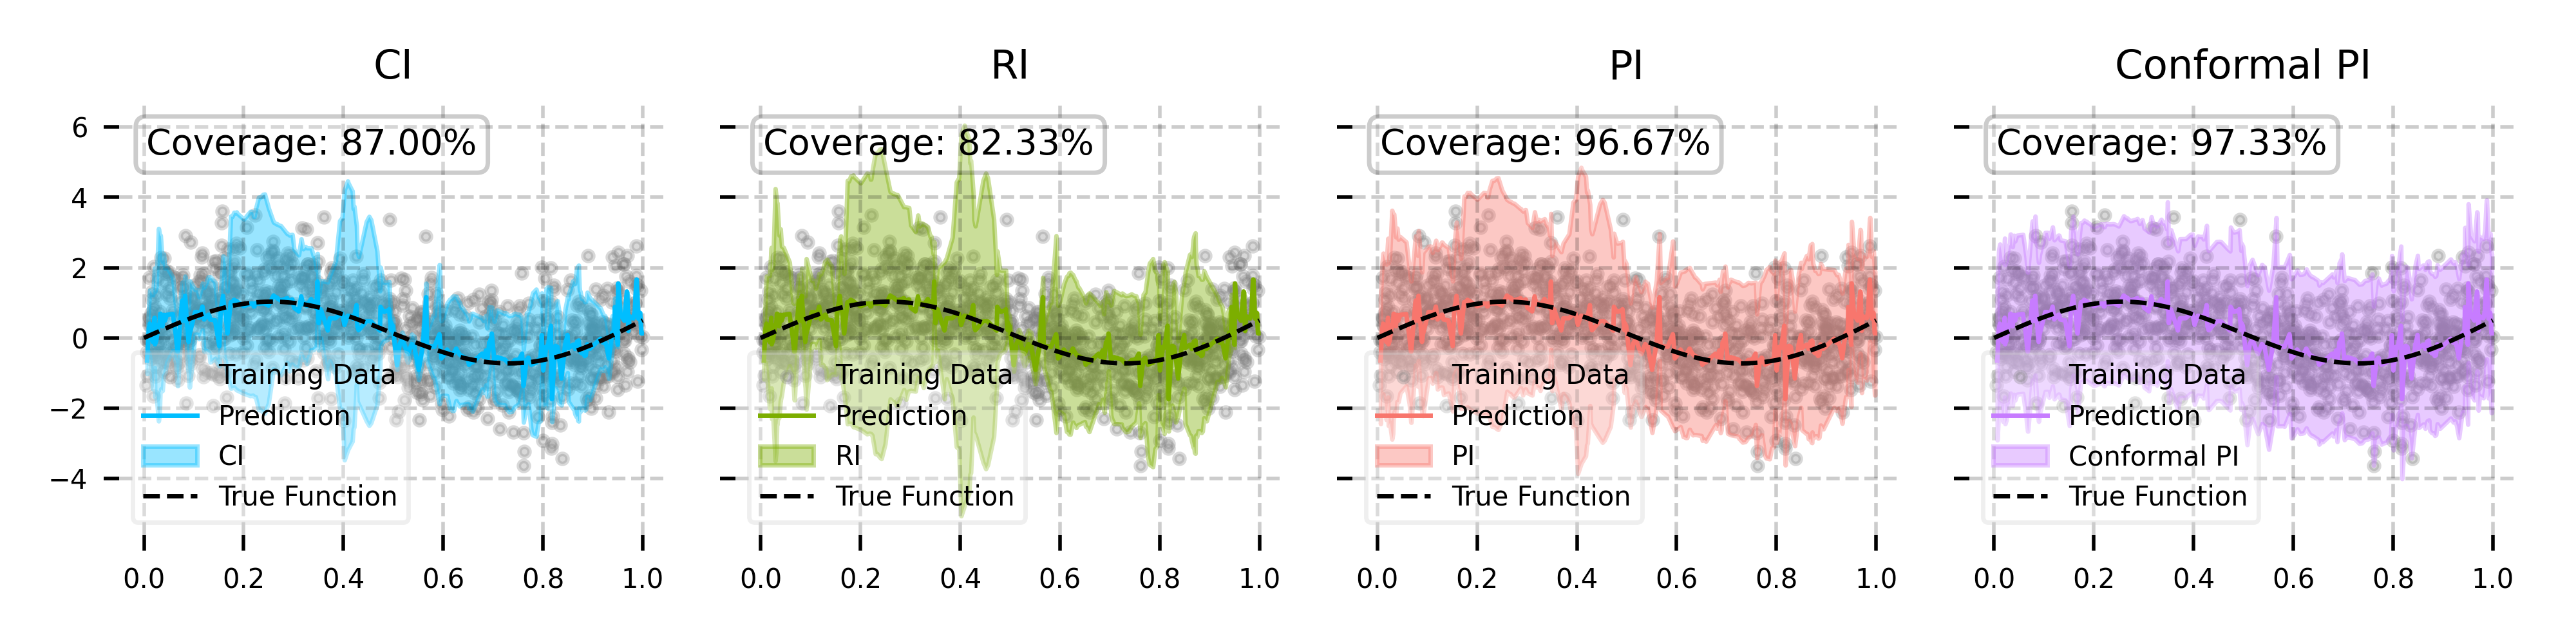
\includegraphics[width=0.9\linewidth]{figures/ch06/plots_gb/1d_coverage.png}
    \vspace{-2ex}
    \caption{Demonstration of confidence, prediction, and reproduction intervals on $\f(x)=\sin 2\pi x + \frac{1}{2} x^2$. Conformal baseline. $200$ trees, learning rate $0.6$, depth $8$, subsampling and dropout $0.6$.}
    \label{fig:1d-coverage}
    \vspace{-2ex}
\end{figure}

\vspace{-1ex}
\textbf{Theoretical contributions.} Our primary theoretical contributions are central limit theorems (CLTs) for boosting with dropout (Algorithm \ref{alg:random-dropout}) and parallel training (Algorithm \ref{alg:structured-dropout}) -- the first such results for these settings to our knowledge. These extend the theoretical arguments of \cite{zhou2022boulevard}. In analyzing boosting with dropout, the stochasticity introduced into ensemble construction must be accounted for -- in addition to randomness from data subsampling. To address this, we establish a weak law for finite-sample convergence in the stochastic contraction framework of \cite{almudevar2022stochasticcontractionmappingtheorem}. 
The arguments for parallel boosting are more challenging. Inspired by classical backfitting methods \citep{breiman1985backfitting}, we develop a delayed averaging scheme that enables parallelism while preserving convergence guarantees. To achieve central limit theorems that hold unconditionally on the data $\bX$, we show a bound on the maximal leaf size is sufficient to limit the influence of distant points and promote balanced splits, enabling rigorous distributional results.

\textbf{Numerical experiments.} We establish the efficacy of our methods on both a simulation study and real-world datasets. Our numerical experiments showcase that our algorithms can be tuned to interpolate between regularized boosting and random forests, and are highly competitive in terms of MSE. These also demonstrate the correctness, coverage, and computational efficiency of the statistical procedures we construct via the central limit theorems our algorithms enjoy.


% First, we are concerned with predictive inference via constructing prediction intervals on (potentially unseen) labels $\by$. Second, we perform statistical inference on the underlying ground truth function $\f$ by constructing confidence intervals for $\f(\bX)$ given $\bX$. Third, we wish to quantify the aleatoric uncertainty within the boosting procedure by constructing what is called reproduction intervals \citep{zhou2022boulevard} for another realization of $\widehat{\f}$ given another independent realization of the training set. Lastly, we also wish to perform hypothesis testing for variable importance (can we omit a feature?) and feature interactions. In summary:


\vspace{-1ex}
\subsection{Setup}
\label{sec:setup}
\vspace{-1ex}

Consider boosting for nonparametric regression with squared error loss. Given random features $\bx \in [0,1]^d$, labels $y \in \R$, and noise $\epsilon \sim \text{SubG}(0,\sigma^2)$, say there exists some function $\f$ such that $y = \f(\bx) + \epsilon$. The learner is given a training set $(\bX^{\train}, \by^{\train})$ of size $n$, and learns an estimate $\widehat{\f}$ of $\f$ by minimizing the mean squared error (MSE) $\frac{1}{n} \sum_{i=1}^n (\widehat{\f}(\bx_i) - y_i)^2$ over the training set. It is customary to analyze how $\widehat{\f}$ converges to $\f$, or in other words, the generalization error of $\widehat{\f}$ on a test set $(\bX^{\test}, \by^{\text{test}})$. Subscripts $\widehat{\f}_n^{(b)}$ indicate the estimated predictor trained on $n$ datapoints for $b$ boosting rounds, where we omit dependencies on $b$ and $n$ whenever possible.

\vspace{-1ex}
\paragraph{Regularized stochastic gradient boosting.} \cite{zhou2022boulevard} propose a regularization procedure called Boulevard that recovers a central limit theorem for boosting. They do so by showing that the resulting regularized procedure converges to a kernel ridge regression. At each iteration
\begin{tightcenter}
    $\textstyle{b=1,...,B-1, \text{ instead of } \widehat{\f}^{(b+1)} \gets \widehat{\f}^{(b)} + \lambda \bt^{(b)}, \text{ they update } \widehat{\f}^{(b+1)} \gets \frac{b-1}{b} \widehat{\f}^{(b)} + \frac{\lambda}{b} \bt^{(b)}}$
\end{tightcenter}
\vspace{-1.2ex}
for the current function estimate $\widehat{\f}^{(b)}$, built tree $\bt^{(b)}$, and learning rate $\lambda \in [0,1)$. As this is equivalent to updating $\widehat{\f}^{(b+1)} \gets \frac{\lambda}{b} \sum_{i=1}^b \bt^{(i)}$, the resulting ensemble is an average of trees. This observation, along with assumptions on tree adaptivity, allows them to prove that Boulevard predictions are asymptotically normal, though they do not construct confidence or prediction intervals. Additionally, this regularization comes at a cost. It turns out that $\widehat{\f}_n^{(b)}$ converges only to $\frac{\lambda}{1+\lambda} \f \leq \f / 2$ as $n,b \to \infty$, and so \emph{Boulevard recovers at most half the signal}. Still, this is the only method available for frequentist inference for gradient boosting, and so we seek to improve upon it in this paper.
\vspace{-2ex}
\begin{figure}[H]
\centering
    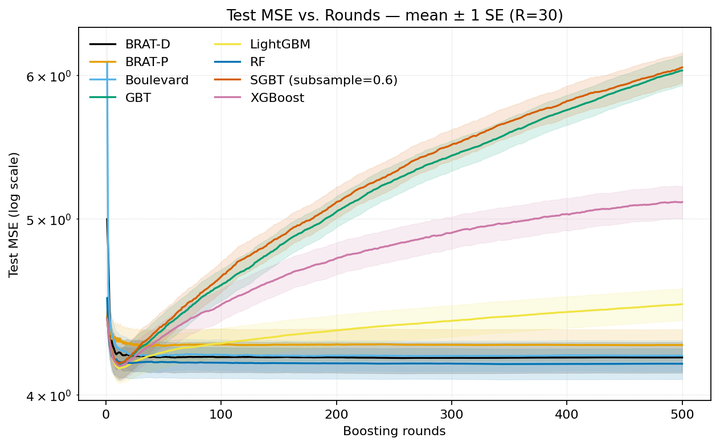
\includegraphics[width=0.49\linewidth]{figures/ch06/plots_gb/camera/mse.png}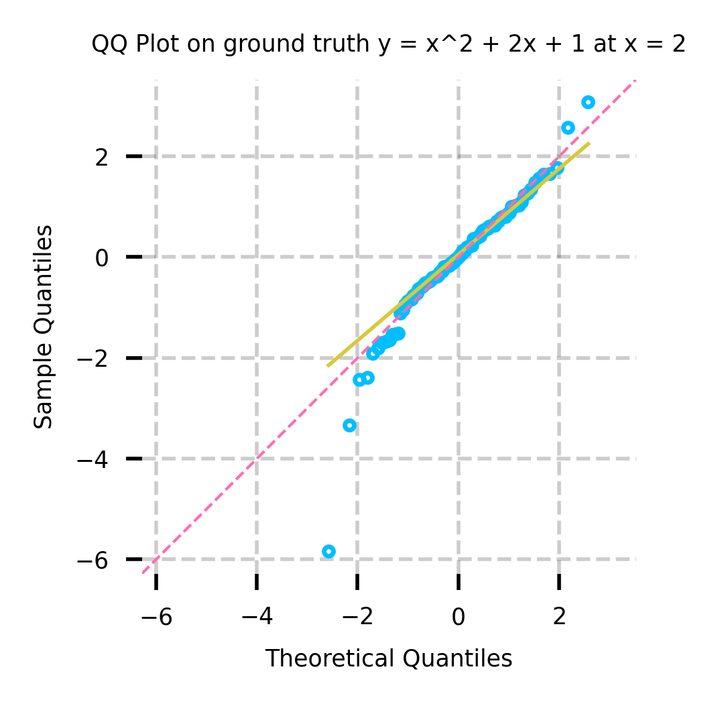
\includegraphics[width=0.32\linewidth]{figures/ch06/plots_gb/camera/qqplot.png}
    \vspace{-1ex}
    \caption{An added benefit of Boulevard regularization is that it renders early stopping unnecessary. Because the procedure converges to a fixed point, one can (in theory) boost indefinitely without encountering overfitting. It also produces asymptotically normal predictions (see the Q-Q plot).}
    \label{fig:no-need-early-stopping}
\end{figure}
\vspace{-2ex}

\vspace{-2ex}
\paragraph{Regression trees and tree structure.} We are primarily concerned with boosting algorithms where we use regression trees as weak learners. We introduce a formulation of a regression tree below.
\begin{defn}[Regression trees]
A regression tree $\bt_n$ trained on $n$ datapoints segments the covariate space $[0,1]^d$ into a partition of hyper-rectangles $\{A_i\}_{i=1}^m$. When $A(\bx)$ for the rectangle containing $\bx$, and $s_{n,j}(\bx)$ is the frequency at which training point $\bx_j$ and test point $\bx$ share a leaf: 
\begin{tightcenter}
    $\textstyle{s_{n,j}(\bx) = \frac{\mathbbm{1}(\bx_j \in A(\bx))}{\sum_{k=1}^n \mathbbm{1}(\bx_k \in A(\bx))}, \text{ the regression tree } \bt_n \text{ predicts }
\bt_n(\bx) = \sum_{j=1}^n s_{n,j}(\bx)\cdot y_j}.$
\end{tightcenter}
\label{defn:regression-trees}
\end{defn}
\vspace{-1ex}
As such, a tree can be thought of as an adaptive nearest neighbor method \citep{athey2018generalizedrandomforests, friedberg2021locallinearforests}, where $s_{n,j}(\bx)$ yields the influence of datapoint $\bx_j$ on the tree's prediction at test point $\bx$. This motivates the definition of a structure vector and matrix from \cite{zhou2022boulevard}:
\vspace{-2ex}
\begin{defn}[Structure vectors and matrices]
    Let $\bt_n$ be a tree trained on the input $(\bX_n, \by_n)$. For an arbitrary point $\bx$, let $\bs_n(\bx) = (s_{n,1}(\bx),...,s_{n,n}(\bx))^\top$ be the structure vector of $\bx$. As such, we say that the matrix $\bS_n = \left(s_{n,j}(\bx_i)\right)_{i,j=1}^n$ with rows $\bs_n(\bx_i)^\top$ is the structure matrix of $\bt_n$.
    \label{defn:structure-matrix}
\end{defn}
\vspace{-1ex}
The structure matrix is a kernel matrix. A natural idea is to perform kernel ridge regression (KRR):
$$\widehat{\f}_n(\bx) = \langle\br_n(\bx), \by_n\rangle, \text{ } \bk_n(\bx) = \E[\bs_n(\bx)], \; \bK_n = \E[\bS_n], \text{ and } \br_n(\bx)^\top = \bk_n(\bx)^\top (\lambda^{-1}\bI + \bK_n)^{-1}.$$
\cite{zhou2022boulevard} show Boulevard regularization converges to a kernel ridge regression $\widehat{\f}_n(\bx) = \langle \br_n(\bx), \by_n\rangle$ as $b \to \infty$. However, as $\lambda \in (0,1]$, this converges to at most half the signal. We later propose two algorithms in Algorithms \ref{alg:random-dropout} and \ref{alg:structured-dropout}, that converge to $\langle\br_n^D(\bx), \by_n\rangle = \bk_n(\bx)^\top (\lambda^{-1}\bI + q\bK_n)^{-1} \by_n$ and $\langle\br_n^P(\bx), \by_n\rangle = \bk_n(\bx)^\top (\bI + (K-1)\bK_n)^{-1}K \by_n$ respectively, achieving increased signal recovery. 
As a final note, to accommodate training $\bt_n(\bx, \gG)$ on a subsample $\gG \subseteq \{1,...,n\}$, we write $s_{n,j}(\bx; \gG) = {\mathbbm{1}(\bx_j \in A, j \in \gG)}/{\sum_{k=1}^n \mathbbm{1}(\bx_k \in A, k \in \gG)}$, and $\bt_n(\bx; \gG) = \sum_{j=1}^n s_{n,j}(\bx;\gG) \cdot y_j$. We suppress the dependence on subsamples when possible.

\vspace{-1ex}
\paragraph{Integrity \& adaptivity.} We inherit the following two assumptions from Boulevard regularization:
\vspace{-2ex}
\begin{aspt}[Structure-value isolation]
\label{aspt:svi}
    $(\bt_n^{(b)})_{b=1}^B$ has $\bs_n^{(b)}(\bx) \indep \by_n$ for all $b=1,...,B$.
\end{aspt}
\begin{aspt}[Non-adaptivity]
\label{aspt:non-adaptivity}
    There exists a probability measure \(\gQ_n\) on the space of tree structures and some $b'$ so the tree structure at iteration $b=b',...,B$ is an independent draw from \(\gQ_n\).
\end{aspt}
\vspace{-1ex}
These are required for theoretical guarantees. In practice, the first can be implemented via a stronger form of honesty \citep{wager2017estimationinferenceheterogeneoustreatment} that we call \emph{integrity}, refitting leaf values on an independent dataset after boosting. One can also randomly sample splits, or get them from a random forest trained on an independent sample. The second only requires non-adaptivity after a finite number of iterations, which may occur naturally \citep{zhou2022boulevard}. To enforce it, one can boost normally for a fixed number of steps and then sample tree structures from earlier iterations. Still, numerical experiments indicate that our algorithms perform well even without these adjustments.


\vspace{-1ex}
\subsection{Algorithms}
\label{sec:algorithms}
\vspace{-1ex}

To address the limitations of Boulevard regularization while retaining its statistical guarantees, we propose two improvements that achieve enhanced signal recovery and improved sample complexity:
\begin{enumerate}[label=\textbf{Alg. \arabic*:}]
    \item By incorporating random dropout \citep{rashmi2015dartdropoutsmeetmultiple} in the ensemble.
    \item By growing trees in parallel within each round with a leave-one-out procedure.
\end{enumerate}
The intuition is as follows. Surprisingly, increasing the dropout probability allows one to recover more of the signal. This is because each tree in the current ensemble is effectively downweighted during residual construction, and the new tree is fit on more of the signal. On the other hand, as the number of trees grown in parallel within each round grows, the resulting ensemble increasingly resembles the procedure of boosting random forests in sequence -- allowing each round to recover more signal than a single tree can. We present both algorithms and explain them in detail below.

\vspace{-2ex}

\begin{algorithm}[H]
    \centering
    \caption{\aigen{Moving-Average Gradient Boosting with Dropout}}
        \begin{algorithmic}[1]
        \STATE \textbf{Input:} Features $\bX$, labels $\by$, dropout rate $p = 1-q$, subsample rate $\xi$, learning rate $\lambda$, boosting rounds $B$. Set $\widehat{\f}^{(0)}, \bt^{(0)} \gets 0$. 
        \FOR{$b=1,...,B-1$}
        \STATE Subsample $\gS_b \subseteq \{0,...,b-1\}$ w.p. $q$.
        \STATE Subsample data $\gG_b \subseteq \{1,...,n\}$ w.p. $ \xi$.
        \STATE
        $z_i \gets y_i - \frac{\lambda}{b}\sum_{s \in \gS_b}\bt^{(s)}(\bx_i)$.
        \STATE Construct tree $\bt^{(b)}$ on $(\bx_i, z_i)_{i \in \gG_b}$.
        \STATE $\widehat{\f}^{(b+1)} \gets \frac{b-1}{b}\widehat{\f}^{(b)} + \frac{\lambda}{b}\bt^{(b)} = \frac{\lambda}{b}\sum_{i=1}^b \bt^{(i)}$.
        \ENDFOR
        \STATE \textbf{Return} final predictor $\frac{1+\lambda q}{\lambda} \widehat{\f}^{(B)}$.
    \end{algorithmic}
    \label{alg:random-dropout}
\end{algorithm}

\begin{algorithm}[H]
    \centering
    \caption{\aigen{Parallel Moving-Average Gradient Boosting with Leave-One-Out Residuals}}
        \begin{algorithmic}[1]
        \STATE \textbf{Input:} Features $\bX$, labels $\by$, subsample $\xi$, trees/round $K$, rounds $B$. $\widehat{\f}^{(0)}, \bt^{(0,k)} \gets 0$. 
        \STATE Fit $\widehat{\f}^{(1)}, (\bt^{(1,k)})_{k=1}^K$ with $K$ boosting steps. 
        \FOR{$b=2,...,B-1$}
        \FOR{$k=1,...,K$ \textbf{in parallel}}
        \STATE Subsample $\gG_{b,k} \subseteq \{1,...,n\}$ w.p. $ \xi$.
        \STATE \hspace{-1.1mm} $z_{i,k} \gets y_i - \frac{1}{b-1}\sum_{s=1}^{b-1}\sum_{l\neq k}\bt^{(s,l)}(\bx_i)$
        \STATE Construct tree $\bt^{(b,k)}$ on $(\bx_i, z_{i,k})_{i \in \gG_{b,k}}$.
        \ENDFOR
        \STATE Define $\widehat{\f}^{(b+1)} \gets \frac{1}{b}\sum_{s=1}^{b}\sum_{k=1}^K \bt^{(s,k)}$.
        \ENDFOR
        \STATE \textbf{Return} final predictor $\widehat{\f}^{(B)}$.
    \end{algorithmic}
    \label{alg:structured-dropout}
\end{algorithm}% \kevin{What is the intuition for why the leave-one-out procedure is enough? Is it simply that 1/K turns out to be the right dropout probability, and it suffices to do it in a derandomized way?}

%\kevin{We can divide by $K$ in each round of parallel boosting to boost random forests. }
\vspace{-1ex}
\paragraph{Random dropout.} Unlike vanilla boosting, Algorithm \ref{alg:random-dropout} computes residuals with both data \citep{friedman2002stochasticboosting} and ensemble subsampling \citep{rashmi2015dartdropoutsmeetmultiple}. At each round $b=1,...,B-1$, each tree is subsampled with a dropout rate of $p \in [0,1)$ (equivalently, with probability $q=1-p$). We write $\gS_b \subseteq \{0,...,b-1\}$ for the collection of subsampled tree indices at each round $b$. Likewise, data indices $\gG_b \subseteq \{1,...,n\}$ are subsampled with probability $\xi \in (0,1]$. 

As a result, each tree $\bt^{(b)}$ is trained on the dataset $(\bx_i, z_i)_{i \in \gG_b}$, where the residuals are given by $z_i = y_i - \frac{1}{b} \sum_{s \in \gS} \bt^{(s)}(\bx_i)$. Within the residual computation, we intentionally divide the sum of the subsampled ensemble's predictions by $b$ instead of $|\gS|$. This is done so each new tree is fit on more of the signal, allowing for increased signal recovery when applying Boulevard regularization. 

We later show in Section \ref{sec:theory} that the predictions of Algorithm \ref{alg:random-dropout} converge to a kernel ridge regression that enjoys a central limit theorem. Informally, for any test point $\bx$, we have that:
$$\textstyle{\widehat{\by}^{(b)}_n \underset{b\to\infty}{\overset{a.s.}{\longrightarrow}} \left(\lambda^{-1} \bI+q \mathbb{E}\left[\bS_n\right]\right)^{-1} \mathbb{E}\left[\bS_n\right]\by_n, \quad\lVert\br_n^D(\bx)\rVert_2^{-1}\left(\widehat{\f}_n^D(\bx) - \frac{\lambda}{1+\lambda q}\f(\bx)\right) \underset{n\to\infty}{\overset{d}{\longrightarrow}} \gN(0, \sigma^2)},$$
for a kernel matrix induced by the tree ensemble $\bK_n = \E[\bS_n]$, and limit $\widehat{\f}_{n}^D = \lim_{b \to \infty} \widehat{\f}^{(b)}_{n}$ where $\widehat{\f}_n^D(\bx) = \langle\br_n^D(\bx),  \by_n\rangle = \bk_n(\bx)^\top (\lambda^{-1}\bI + q\bK_n)^{-1}\by_n$. $\lVert\br_n\rVert_2$ is the norm of kernel weights. Algorithm \ref{alg:random-dropout} encompasses two important special cases. When $\lambda=1$ and $p\to 1$, this yields a random forest. When $p=0$, Algorithm \ref{alg:random-dropout} corresponds to the original Boulevard algorithm \citep{zhou2022boulevard}. Tuning the dropout parameter $p$ allows the user to interpolate between the two, while improving over \cite{zhou2022boulevard} by up to a factor of $\frac{1+\lambda}{1+\lambda q} \in (1, 2]$ in signal recovery.%\footnote{This improvement is maximized when $\lambda=1$ and $p=1$. Observe that the rescaling factor necessary to achieve consistency $\lambda^{-1}(1+\lambda q)$ goes to $1$ as both the learning and dropout rates go to $1$.}



\vspace{-2ex}
\paragraph{Parallel boosting.} Algorithm \ref{alg:structured-dropout} integrates a novel leave-one-out procedure and Boulevard regularization into the parallel boosting framework \citep{long2011parallelmargin, karbasi2023impossibilityparallelizingboosting, dacunha2024optimalparallelizationboosting}. The algorithm is warm-started by performing $K$ vanilla boosting iterations in the first round. At each subsequent round $b=2,...,B-1$, we grow $K$ trees $(\bt^{(b,k)})_{k=1}^K$ in parallel on the $K$ datasets $((\bx_i, z_{i,k})_{i \in \gG_{b,k}})_{k=1}^K$. These consist of independently subsampled data indices $\gG_{b,k} \subseteq \{1,...,n\}$, and residuals that are computed by leaving one ``column'' out (or alternatively, one tree out per round): $z_{i,k} = y_i - \frac{1}{b-1}\sum_{s=1}^{b-1}\sum_{l\neq k}\bt^{(s,l)}(\bx_i)$. The resulting predictor is given by the regularized boosting update: $\widehat{\f}^{(b+1)} \gets \frac{b-1}{b} \widehat{\f}^{(b)} + \frac{1}{b} \sum_{k=1}^K \bt^{(b,k)} = \frac{1}{b}\sum_{s=1}^{b}\sum_{k=1}^K \bt^{(s,k)}$.
%\footnote{This can be thought of as a \emph{structured} variant of dropout \citep{zhao2022revisitingstructureddropout, xin2020deebertdynamicearlyexitingdropout, fan2019reducingtransformerdepthdemanddropout}. Dropping one out of every $K$ trees allows the regularization to scale in $1/K$.}

Likewise, we later show in Section \ref{sec:theory} that the predictions of Algorithm \ref{alg:structured-dropout} also converge to a kernel ridge regression that enjoys a central limit theorem. Informally, for any test point $\bx$:
$${\widehat{\by}^{(b)}_n \underset{b\to\infty}{\overset{a.s.}{\longrightarrow}} \left(\bI+ (K-1)\mathbb{E}\left[\bS_n\right]\right)^{-1} K\mathbb{E}\left[\bS_n\right]\by_n, \quad \lVert\br_n^P(\bx)\rVert_2^{-1}\left(\widehat{\f}_n^P(\bx) - \f(\bx)\right) \underset{n\to\infty}{\overset{d}{\longrightarrow}} \gN(0, \sigma^2)},$$
with limit $\widehat{\f}_{n}^P = \lim_{b \to \infty} \widehat{\f}^{(b)}_{n}$ given by $\widehat{\f}_{n}^P(\bx)= \langle\br_n^P(\bx), \by_n\rangle = \bk_n(\bx)^\top (\bI + (K-1)\bK_n)^{-1}K \by_n$. 
Algorithm \ref{alg:structured-dropout} can be viewed as boosting a modified parallel backfitting algorithm \citep{breiman1985backfitting}\footnote{This can be thought of as a \emph{structured} variant of dropout \citep{zhao2022revisitingstructureddropout, xin2020deebertdynamicearlyexitingdropout, fan2019reducingtransformerdepthdemanddropout}. Dropping one out of every $K$ trees allows the regularization to scale in $1/K$.} that is warm-started with $K$ vanilla boosting iterations.\footnote{The initial $K$ boosting iterations yield better convergence in practice, and do not hinder our theoretical arguments as the impact of the vanilla boosting iterations washes out when we take $B \to \infty$.} When $K=1, B\to\infty$, Algorithm \ref{alg:structured-dropout} reduces to a random forest $\mathbb{E}\left[\bS_n\right]\by_n$. On the other hand, Algorithm \ref{alg:structured-dropout} reduces to vanilla boosting when $B=1, K\to\infty$. Note that the CLT only holds for $1 < K < \infty$. 

The attentive reader may observe that we do not divide the final predictions by $K$. This is because the combination of leaving one column out when fitting a tree and Boulevard averaging is sufficient to allow our procedure to stabilize.\footnote{Parallelized backfitting can be thought of as parallelized coordinate descent. Averaging over the coordinate updates is sufficient for convergence. Dividing by $b$, as in Boulevard averaging, is sufficient when $b \geq K$.} Still, dividing by $K$ yields a viable algorithm (deferred to future work) that can be thought of as boosting random forests each of $K$ trees over $B$ rounds, using the natural strategy of averaging all trees but the left-out column to form predictions. 

% \newpage
% Do you mean
% $$\widehat{f}^{(b+1, k)} = \frac{1}{b}\sum_{s=1}^{b}\sum_{l=1}^{k}t^{s,l} + \frac{1}{b-1}\sum_{s=1}^{b-1}\sum_{l=k+1}^{K}t^{s,l}?$$

% If so, this is almost 
% $$\widehat{f}^{(b+1)} = \frac{1}{b}\sum_{s=1}^{b}\sum_{k=1}^K t^{s,k},$$
% which is equivalent to 
% $$\widehat{\f}^{(b+1)} \gets \frac{b-1}{b} \widehat{\f}^{(b)} + \frac{1}{b} \sum_{k=1}^K \bt^{(b,k)} = \frac{1}{b}\sum_{s=1}^{b}\sum_{k=1}^K \bt^{(s,k)}.$$

% $\widehat{f}^{(b, k+1)} = \frac{1}{b}\sum_{s=1}^{b}\sum_{l=1}^{k+1}t^{s,l} + \frac{1}{b-1}\sum_{s=1}^b\sum_{l=k+2}^{K}t^{s,l}$


\vspace{-1ex}
\subsection{Statistical Inference and Uncertainty Quantification for Boosting}
\label{sec:statistics}
\vspace{-1ex}

We are now in a place to introduce our methods for conducting statistical inference for boosting; theoretical basis for these procedures is provided below. Our methods rest on the aforementioned convergence to a kernel ridge regression and central limit theorems that we formally prove later in Theorems \ref{thm:krrconv} and \ref{thm:main}. In the meantime, we provide the following asymptotically valid procedures.


\vspace{-1ex}
\paragraph{Estimation of asymptotic variance.} The CLTs for Algorithms \ref{alg:random-dropout} and \ref{alg:structured-dropout} imply that one can construct confidence intervals for $\f$ with the following normal approximations:
$$\lambda^{-1}(1+\lambda q)\widehat{\f}_n^D(\bx) \stackrel{d}{\approx} \gN\left(\f(\bx), \lambda^{-2}(1+\lambda q)^2\lVert\br_n^D(\bx)\sigma^2 \rVert_2^2 \right), \;\; \widehat{\f}_n^P(\bx) \stackrel{d}{\approx} \gN\left(\f(\bx), \sigma^2 \lVert\br_n^P(\bx)\rVert_2^2\right).$$
As such, it remains to estimate $\br_n^D, \br_n^P$, and $\sigma^2$. We first estimate $\bk_n(\bx)$ by the sample averages
\begin{equation}
    \textstyle{\widehat{\bk}_n^D(\bx) = \frac{1}{B} \sum_{b=1}^B s_{n,i}^{(b)}(\bx, \gG_b),\;\; \widehat{\bk}_n^P(\bx) = \frac{1}{BK} \sum_{b=1}^B \sum_{k=1}^K s_{n,i}^{(b,k)}(\bx, \gG_{b,k}),}
    \label{eqn:hat-k}
\end{equation}
%s_{n,i}^{(b)}(\bx; \gG_b) = \frac{\mathbbm{1}(\bx_k \in A_j^{(b)}, k \in \gG_b)}{\sum_{i=1}^n \mathbbm{1}(\bx_i \in A_j^{(b)}, i \in \gG_b)}
where $s_{n,i}^{(b)}(\bx; \gG_b)$ is the fraction of subsampled datapoints in the same leaf $A_j^{(b)}$ as $\bx$ over the trees. Likewise, we estimate $(\bK_n)_{i,j}$, the fraction of trees where datapoints $i$ and $j$ fall in the same leaf:
\begin{equation}
    \textstyle{(\widehat{\bK}_n^D)_{i,j} = \frac{1}{B} \sum_{b=1}^B s_{n,j}^{(b)}(\bx_i; \gG_b), \;\;(\widehat{\bK}_n^P)_{i,j} = \frac{1}{B} \sum_{b=1}^B s_{n,j}^{(b,k)}(\bx_i; \gG_{b,k})},
    \label{hat-K}
\end{equation}
Our estimates of $\widehat{\br}_n$ are then given by plugging the above into the formula for $\br_n$:
$$\widehat{\br}_n^D(\bx)^\top = \widehat{\bk}^D_n(\bx)^\top (\lambda^{-1}\bI + q\widehat{\bK}^D_n)^{-1}, \;\;\widehat{\br}_n^P(\bx)^\top = \widehat{\bk}^P_n(\bx)^\top (\bI + (K-1)\widehat{\bK}^P_n)^{-1}K.$$
Lastly, we estimate $\sigma^2$ with the residuals $\widehat{\sigma}^2 = \frac{1}{n_{\text{cal}}}\sum_{i=1}^{n_{\text{cal}}} (y_i - \widehat{y}_i)^2$ on a hold-out calibration set. We describe a tweak later in Section \ref{sec:coverage-experiments} that uses the calibration set for increased robustness.

\vspace{-1ex}
\paragraph{Confidence intervals for $\f$.} Putting everything together yields $1-\alpha$ confidence intervals for $\f$ (where $z_{1-\alpha/2}$ is the $(1-\alpha/2)$-quantile of the standard normal distribution):
\begin{equation}
    \lambda^{-1}(1+\lambda q)\widehat{\f}_n^D(\bx) \pm z_{1-\alpha/2}\lambda^{-1}(1+\lambda q)\widehat{\sigma}\lVert\widehat{\br}_n^D(\bx)\rVert_2 ,\;\; \widehat{\f}_n^P(\bx) \pm z_{1-\alpha/2} \widehat{\sigma}\lVert\widehat{\br}_n^P(\bx)\rVert_2.
    \label{eqn:confidence-intervals}
\end{equation}


\vspace{-1ex}
\paragraph{Prediction intervals for $\by$.} We can construct prediction intervals for $y | \bx$ as follows:
\begin{equation*}
    \lambda^{-1}(1+\lambda q)\widehat{\f}_n^D(\bx) \pm z_{1-\alpha/2}\lambda^{-1}(1+\lambda q)\widehat{\sigma}\sqrt{1+\lVert\widehat{\br}_n^D(\bx)\rVert_2^2},\;\; \widehat{\f}_n^P(\bx) \pm z_{1-\alpha/2} \widehat{\sigma}\sqrt{1+\lVert\widehat{\br}_n^P(\bx)\rVert_2^2}.
    \label{eqn:prediction-intervals}
\end{equation*}
These prediction intervals have asymptotic pointwise coverage, conditional on the test point $\bx$. That is, $\prob(y \in \text{PI}(\bx) | \bx) \to 1-\alpha$ as $n \to \infty$, which holds as a corollary of the CLTs we present in the following section. Note that this conditional coverage guarantee is a stronger guarantee than is typically possible with conformal inference \citep{barber2020limitsdistributionfreeconditionalpredictive}. We compare our prediction intervals to conformal prediction intervals within our numerical experiments later in this paper.


\vspace{-1ex}
\paragraph{Reproduction intervals for $\widehat{\f}$.} We now turn our attention towards computing reproduction intervals. That is, a confidence interval for another realization of $\widehat{\f}$ trained on another independent realization of the data. To do so, as \cite{zhou2022boulevard} suggest, it suffices to scale the width of the above confidence intervals for $\f$ by $\sqrt{2}$ as $X_1, X_2 \stackrel{i.i.d.}{\sim} \gN(0,\sigma^2) \implies X_1 - X_2 \sim \gN(0,2\sigma^2)$.
Note that one can invert the above confidence, prediction, or reproduction intervals in order to test if the underlying function, another realization of the response, or average learner is equal to a given constant. This amounts to checking if the constant is contained in the interval of choice. 

%\kevin{Ziang thinks that because our kernel is effectively a nearest neighbor kernel, our kernel method may inherit the same adaptiveness to intrinsic dimensionality that nearest neighbors does. See https://luc.devroye.org/Biau+Devroye-LecturesontheNearestNeighborMethod-2015.pdf.}

\vspace{-1ex}
\paragraph{Variable importance tests.} Suppose we wish to test for variable importance. Consider the possibility that there exists some subset of the feature space $[0,1]^d$ containing only $\widecheck{d} < d$ features, and let $\g : [0,1]^{\widecheck{d}} \to \R$ be the projection of $\f$ onto $\gL^2([0,1]^{\widecheck{d}})$. We test the possibility that $\f(\bx) = \g({\bx})$ by proxy. Consider a split of the training dataset $(\bX_n, \by_n)$ into $(\bX_{n,1}, \by_{n,1}), (\bX_{n,2}, \by_{n,2})$, where $\bX_{n,1} \in \R^{n/2, d}, \bX_{n,2} \in \R^{n/2,\widecheck{d}}$. Let $\widehat{\f}_{n,1}$ be the boosting learner trained on $(\bX_n, \by_n)$, and $\widehat{\f}_{n,2}$ be the same trained on $({\bX}_{n,2}, \by_{n,2})$. Given a hold-out dataset $(\bX_m, \by_m)$, we test the null:
$$H_0 : \f(\bx_j) = \g({\bx}_j) \text{ for all } j=1,...,m \text{ against } H_1 : \f(\bx_j) \neq \g({\bx}_j) \text{ for some } j$$
by comparing $\widehat{\f}_{n,1}(\bx_j)$ and $\widehat{\f}_{n,2}({\bx}_j)$. We exploit the CLTs our algorithms enjoy to do so. Write $\widehat{\br}^{D,P}_n(\bX_m)^\top \in \R^{m \times n}$ for the matrix with rows $(\widehat{\br}^{D,P}_n(\bx_l)^\top)_{l=1}^m$, where we write $D,P$ within the superscript if the formula holds for both Algorithms \ref{alg:random-dropout} and \ref{alg:structured-dropout}. The difference in predictions 
$$\widehat{\d}_m = (\widehat{\br}^{D,P}_{n,1}(\bX_m) - \widehat{\br}^{D,P}_{n,2}(\bX_m))^\top \by \; \stackrel{d}{\to} \; \gN_m(\mathbf{0}, \sigma^2 \widehat{\bXi}_n) \text{ is multivariate normal under the null},$$
with covariance matrix $\sigma^2 \widehat{\bXi}_n = \sigma^2 (\widehat{\br}^{D,P}_{n,1}(\bX_m) - \widehat{\br}^{D,P}_{n,2}(\bX_m))^\top (\widehat{\br}^{D,P}_{n,1}(\bX_m) - \widehat{\br}^{D,P}_{n,2}(\bX_m))$ estimated by plugging in $\widehat{\sigma}^2$. As such, we can conduct a chi-squared test with test statistic
$$\widehat{\sigma}^{-2} \widehat{\d}_m^\top \widehat{\bXi}_n^{-1} \widehat{\d}_m \sim \chi_m^2 \text{ under the null}, \text{ rejecting the null if } \widehat{\sigma}^{-2} \widehat{\d}_m^\top \widehat{\bXi}_n^{-1} \widehat{\d}_m > \chi_{m,1-\alpha}^2.$$
The test as presented runs in $O(n^3)$ time. In Appendix \ref{app:random-projections}, we present an accelerated version of the test that runs in 
$O(ns(r+s) + r^3)$ time, where $s$ is the number of points subsampled for Nystr\"{o}m approximation and $r$ is the number of test points subsampled. 

%Our results extend the tests developed in \cite{mentch2016randomforestci} to the boosting setting, but unlike their tests, ours remain computationally efficient and run in linear time in the number of training points, and sublinear time in the number of test points.


% \kevin{Procedure is to build a booster on original training set and another on the restricted training set. The vector of differences in predictions on the hold-out dataset is multivariate normal. Under the null, this is mean zero. The covariance of this vector is not straightforward, but is this given by the covariance of differences in predictions between each tree in the ensemble? That would be the case for a random forest. Not clear if this is the case for regularized boosting. Probably need to work this out in terms of the kernel regressions. }


\vspace{-1ex}
\paragraph{Matrix sketching.} Although he CLT reduces the problem of inference to kernel ridge regression (with the right kernel), computing \(\widehat{\bK}_n\) is an $O(n^3)$ problem -- intractable for large $n$. This is the chief difficulty that Zhou and Hooker (2022) face when constructing replication intervals for vanilla Boulevard.
We bypass this issue, making our procedures practical and tractable via matrix sketching.

We approximate \(\widehat{\bK}_n\) using the Nystr\"{o}m method \citep{williams2000nystromkernel}, via either uniform subsampling or the recursive approach of \cite{musco2017recursivenystrom}, producing an approximation \(\widetilde{\bK}_n \approx \widehat{\bK}_n\bS(\bS^\top \widehat{\bK}_n\bS)^{\dagger} \bS^\top \widehat{\bK}_n\), where \(\bS \in \mathbb{R}^{n \times s}\) is a random subsampling matrix. With the Nystrom method of Musco and Musco (2017), we can choose $s$ to near-linear in the effective dimension $d_{\text{eff}}^\mu$ of a ridge regression problem with regularization parameter $\mu$ on the kernel matrix: $s = \widetilde{O}(d_{\text{eff}}^\mu)$.

This requires only $O(ns^2)$ time to precompute the kernel, and only $O(s^2)$ time for inference -- yielding practical statistical inference in near-linear time in the number of datapoints $n$. We adopt this approach in our experiments, allowing our procedures to run in linear time and remain practical, unlike previous work \citep{zhou2022boulevard, mentch2016randomforestci}. See Appendix \ref{app:random-projections}.





\vspace{-1ex}
\subsection{Theoretical Guarantees}
\vspace{-1ex}
\label{sec:theory}
As promised, we now formally present guarantees for convergence and asymptotic normality for Algorithms \ref{alg:random-dropout} and \ref{alg:structured-dropout}. Consider the (Lipschitz) nonparametric regression model introduced below:
\begin{aspt}[Lipschitz Nonparametric Regression]
    Let \(y = f(\bx) + \epsilon,\) where \(\mathbf{x}\) has density \(\mu\) satisfying $0 < c_1 \le \mu(\mathbf{x}) \le c_2 < \infty$ on its support. Further assume \(f\) is \(\alpha\)-Lipschitz continuous on \(\mathrm{supp}(\mu)\), and noise \(\epsilon\) is sub-Gaussian with variance proxy \(\sigma^2\).
    \label{aspt:nonparametric-regression}
\end{aspt}

\vspace{-1ex}
\paragraph{Finite-sample convergence to KRR.} We now show that our algorithms achieve finite-sample convergence to kernel ridge regression as the number of boosting rounds increases. At first glance, this is surprising -- greedy split selection and sequential ensemble construction create a highly nonlinear and time-dependent mapping. Fortunately, the regularization procedure of \cite{zhou2022boulevard} provides a way forward. 
For the special case of $p=0$ within Algorithm \ref{alg:random-dropout}, they show convergence to a kernel ridge regression via the stochastic contraction framework of \cite{almudevar2022stochasticcontractionmappingtheorem}, utilizing Assumptions \ref{aspt:svi} (structure–value isolation) and \ref{aspt:non-adaptivity} (non-adaptivity) to ensure stagewise stability. 
A key novelty within our analysis lies in showing that this convergence extends to Algorithms \ref{alg:random-dropout} and \ref{alg:structured-dropout}, even with the added complexity introduced by dropout and parallelism respectively. Despite these added sources of stochasticity and dependence, our use of the same regularization mechanism ensures that both algorithms inherit the stability required for convergence:
\begin{thm}[Finite Sample Convergence to KRR]
\label{thm:krrconv}
For fixed $\bX, \by$, under Assumptions \ref{aspt:svi}, \ref{aspt:non-adaptivity}, and \ref{aspt:nonparametric-regression},
$$\widehat{\by}_b \stackrel{\text{a.s.}}{\to} \left(\lambda^{-1} \bI+q \mathbb{E}\left[\bS_n\right]\right)^{-1} \mathbb{E}\left[\bS_n\right] \by \text{ for Alg. \ref{alg:random-dropout}},
\;
\widehat{\by}_b \stackrel{\text{a.s.}}{\to} \left(I+(K-1)\mathbb{E}\left[\bS_n\right]\right)^{-1} K\mathbb{E}\left[\bS_n\right] \by \text{ for Alg. \ref{alg:structured-dropout}},$$
as $b \to \infty$, where $q=1-p$ is one minus the dropout probability, $K$ is the number of trees grown in parallel, and $\bS_n$ is the kernel matrix induced by the tree structures within the ensemble.
\end{thm}
The proof, deferred to Appendix \ref{app:finite-sample-convergence}, departs from \cite{zhou2022boulevard} in two crucial ways. Within Algorithm \ref{alg:random-dropout}, dropout injects unbounded variance into the ensemble updates. To control this, we introduce the hard truncation function $\Gamma_M(y) = \operatorname{sign}(y)\min\{M,|y|\}$ into each residual update,
$
  \widehat{\by}_b 
    = \frac{b-1}{b}\,\widehat{\by}_{b-1}
    + \frac{\lambda}{b}\,\bS_b\bigl(\by - \Gamma_M(\widetilde{\by}_b)\bigr),
$
and then show that the probability of the partial ensemble escaping this cap vanishes as $b\to\infty$. Within Algorithm \ref{alg:structured-dropout}, truncating $\widetilde{\by}_{b,k}=\widehat{\by}_{b-1,K}-\Gamma_M(\frac{1}{b-1}\sum_{g=1}^{b-1}\widehat{\bt}_{b,k})$ alone is insufficient. We further introduce a delay mechanism, requiring that $\bt_{b,k}$ does not rely on $\bt_{b,k-1}$, allowing us to apply Theorem  \ref{thm:stochastic-contraction-mapping} and parallelize tree training. 

\vspace{-1ex}
\paragraph{A central limit theorem.} Having established almost-sure convergence to fixed points, we now examine the asymptotic distribution of our estimators to justify the statistical procedures introduced in Section \ref{sec:statistics}. We seek a central limit theorem for the learner $\widehat{\f}_n^{D,P}$, trained on random $\bX_n, \by_n$, demonstrating that the predictions $\widehat{\f}_n^{D,P}(\bx)$ 
are asymptotically normal with mean $\f(\bx)$ as $n \to \infty$. To do so, we inherit the following assumptions from \cite{zhou2022boulevard}: two on the leaves to control the norm of the KRR weight vector $\br_n^{D,P}$, and a restriction on the tree distribution space:
\begin{aspt}[Bounded Leaf Diameter]
    \label{aspt:leaf-diameter}
    Write $\mathsf{diam}(A)=\sup_{x,y\in A}\norm{x-y}$. For any leaf $A$ in a tree with structure $q\in Q_n$, we need $\sup_{A \in q} \mathsf{diam}(A) =  O(d_n)$, where $d_n = O(n^{-{1}/{(d+1)}})$.
\end{aspt}
\vspace{-1ex}
\begin{aspt}[Increased Minimal Leaf Size]
    \label{aspt:ub-minimal-leaf-size}
    For any $\nu >0$, \(v_n =n^{-\frac{d+1}{d+2}+\nu}<n^{-\frac{d}{d+1}}=O(d_n^d)\).
\end{aspt}
\begin{aspt}[Restricted Tree Support]
    \label{aspt:restricted-tree-space}
    The cardinality of the tree space $Q_n$ is bounded by $O(n^{-1} \exp(0.5 n^{{1}/{(d+2)}-\nu} - n^{\alpha}))$, for some small $\alpha > 0$.
\end{aspt}
\vspace{-1ex}
Intuitively, Assumption \ref{aspt:ub-minimal-leaf-size} prevents leaves from becoming too small too quickly, which in turn controls the maximal coordinate of the weight vectors across random samples. Assumption \ref{aspt:restricted-tree-space}, guarantees that the complexity of possible tree partitions does not explode with \(n\). We also make assumptions on the regularity of tree splits in line with the notion of $\alpha$-regularity in \cite{athey2018generalizedrandomforests}:
\vspace{-1ex}
\begin{aspt}[Median Splitting Rules]
    \label{aspt:median-trees}
    The trees in Algorithm \ref{alg:structured-dropout} are split at the medians.
\end{aspt}
\vspace{-1ex}
We defer the details to Definition \ref{def:alpha_regular}. Under this splitting rule, the point-to-point collision probability is well-controlled, i.e. to say none of the leaves are big enough to contain most of the points. 
These conditions allow for uniform control over both leaf sizes and tree complexity, yielding the result:
\begin{thm}[Central Limit Theorem for Predictions]
	\label{thm:main}
	Let $\bx \in [0,1]^d$, $q \in (0,1]$, $K > 1$. As $n \to\infty$,
	$$
	\norm{\br^D_n}_2^{-1}\left(\widehat{\f}^D_n(\bx) - \lambda^{-1}(1+\lambda q)\f(\bx)\right) \stackrel{d}{\longrightarrow} \mathcal{N}(0,\sigma^2), \quad
	\norm{\br^P_n}_2^{-1}\left(\widehat{f}^P_n(\bx) - f(\bx)\right) \stackrel{d}{\longrightarrow} \mathcal{N}(0,\sigma^2).
	$$
\end{thm}
\vspace{-1ex}
We prove this in two stages. In the first, with proof deferred to Appendix \ref{app:conditional-clt}, we show asymptotic normality of the predictions around the noiseless KRR predictions $\langle \br_n^{D,P}(\bx), \f(\bX_n)\rangle$, conditional on the training data $\bX_n, \by_n$ and test point $\bx$, by applying the Lindeberg-Feller CLT to \(\langle\mathbf{r}_n^{D,P}(\bx), \varepsilon\rangle\). 
Next, we show that $\langle \br_n^{D,P}(\bx), \f(\bX_n)\rangle$ converges to the underlying ground truth function at a sufficiently fast rate in Appendices \ref{app:random-clt} and \ref{app:main-theorem}. For Algorithm \ref{alg:random-dropout}, although $\br_n^D$ now involves $[\frac1\lambda \bI+q\bK_n]^{-1}$, this still preserves the rate $\|\br_n\|_2\asymp n^{-1/(2(d+1))}$, allowing us to show $\langle \br_n,f(\bX_n)\rangle-\frac{\lambda q}{1+\lambda q} \f(\bx)=o_p(\|\br_n\|_2)$. The Lindeberg–Feller verification then proceeds identically to the non‑dropout case. However, to give a CLT for Algorithm \ref{alg:structured-dropout}, controlling the influence from distant training points is challenging, though we show that Assumption \ref{aspt:median-trees} is sufficient to do so. 

\vspace{-1ex}
\paragraph{Understanding the result.} 
The rate of convergence of the CLT in Theorem \ref{thm:main} depends on the norm of $\br_n^{D,P}$. This is controlled as follows, yielding generalization bounds for Algorithms \ref{alg:random-dropout} and \ref{alg:structured-dropout}:
\begin{lem}[Rate of Convergence]
Let $\mathbf{B}_n := \{i  : \norm{\bx-\bx_i}\leq d_n\}$ be the points within distance $d_n$ from test point $\bx$. If $\left| \mathbf{B}_n \right|  = \Ome{ n \cdot d_n^d }$, then
	$
	\norm{\bk_n}_2 = \Theta(n^{-\frac{1}{2}\frac{1}{d+1}}),
    \norm{\br^{D,P}_n}_2 = \Theta(n^{-\frac{1}{2}\frac{1}{d+1}}).
    $
\label{lem:rateofr}
\end{lem}
\begin{cor}
\label{cor:asymptotic-risk}
$
\E[(\frac{1+\lambda q}{\lambda}\widehat{\f}^D_n(\bx)-\f(\bx))^2]
\lesssim (\frac{1+\lambda q}{\lambda})^2\sigma^2 n^{-\frac{1}{d+1}}$ and $ 
\E[(\widehat f^P_n(\bx)-f(\bx))^2]
\lesssim \sigma^2 n^{-\frac{1}{d+1}}.
$
\end{cor}
\begin{cor}
\label{cor:non-asymptotic-risk}
If $n \geq \Omega\left(\frac{\log(1/\delta)}{\epsilon^{d+1}}\right)$, $b \geq \Omega\left(\frac{n\lambda^2M^2}{\epsilon^{2}\delta}\right)$, then w.p. at least $1-\delta$, $|\widehat{\f}_n^{(b)}(\bx) - \f(\bx)| \leq \epsilon$.
\end{cor}
The first is an asymptotic risk bound, while the second is a nonasymptotic PAC guarantee. Recall that $M$ is the truncation level.
The results above recover the minimax rate for nonparametric regression on $1/2$-Holder smooth functions \citep{stone1982} -- quadratically worse than the rate for Lipschitz functions (the setting we are in). We believe this can be improved -- trees should inherit adaptivity to the intrinsic dimension as an adaptive nearest neighbor method, but we leave this for future work.


Furthermore, Theorem \ref{thm:main} yields asymptotic coverage of our intervals constructed in Section \ref{sec:statistics}:
\begin{cor}
    \label{cor:cov-rate}
    The CIs, PIs and RIs achieve $1-\alpha$ almost sure pointwise coverage as $n,b \to \infty$.
\end{cor}

We show in Lemma \ref{lem:rateofr} that the rate at which $\lVert\br_n^{D,P}\rVert_2$ grows is the same for Algorithms \ref{alg:random-dropout} and \ref{alg:structured-dropout}. This shows that our methods achieve an asymptotic relative efficiency relative to \cite{zhou2022boulevard} by up to a factor of $4$ for Algorithm \ref{alg:random-dropout}, and at least a factor of $4$ for Algorithm \ref{alg:structured-dropout}:
\begin{cor}[Asymptotic Relative Efficiency]
    \label{cor:are}
    Write $\widehat{\f}^B$ for the scaled predictions made by vanilla Boulevard \citep{zhou2022boulevard} with the same learning rate $\lambda \in (0,1]$ as Algorithm \ref{alg:random-dropout}. Then,
    \begin{tightcenter}
        $
    {\text{Var}(\frac{1+\lambda}{\lambda}\widehat{\f}^B)}/{\text{Var}(\frac{1+\lambda q}{\lambda}\widehat{\f}^D)}=(\frac{1+\lambda}{1+\lambda q})^2 \in [1,4],
    \; 
    {\text{Var}(\frac{1+\lambda}{\lambda}\widehat{\f}^B)}/{\text{Var}(\widehat{\f}^P)}=\left(\frac{1+\lambda}{\lambda}\right)^2 \in [4,\infty).
    $
    \end{tightcenter}
\end{cor}
\vspace{-2ex}
This has the implication that Algorithms \ref{alg:random-dropout} and \ref{alg:structured-dropout} achieve increased signal recovery in the square root of the ARE relative to vanilla Boulevard. The intuition for this improvement is as follows. For any choice of $\lambda$ within vanilla Boulevard, there exists a choice of $p$ within Algorithm \ref{alg:random-dropout} that requires a smaller rescaling. On the other hand, as Algorithm \ref{alg:structured-dropout} requires no rescaling, it can achieve an unbounded improvement in relative efficiency over vanilla Boulevard as we take $\lambda \to 0$.

% \haimo{Write out the actual rate of $\norm{\br_n}$. Also need non-asymptotic risk }. \kevin{Potential extension to bounding the risk in terms of the intrinsic dimension of the data. Trees likely enjoy this property with the right splitting method. }
% Another lemma on the ARE of both algorithms with respect to vanilla Boulevard \cite{zhou2022boulevard} can be shown.

% Convenient inference tools allowed by our CLTs are confidence intervals, prediction intervals and reproduction intervals. \haimo{Should we also incorporate conformal here? Do we need to prove that? This seems straightforward cuz in the simulation the models are not only exchangeable but also independent.} \kevin{lol no. conformal is just something we use as a benchmark. it's very general anyway so guarantees should apply regardless of whether we prove anything or not. we expect it to have coverage but be a mile wide} Denote the variance made by our models as \(\sigma_D^2:=(\frac{1+\lambda q}{q})^2\norm{r_n^D}^2\sigma^2, \sigma_P^2=\norm{r_n^P}^2\sigma^2\). Given $\forall \bx \in [0,1]^d$. Formally, intervals are given by:
% \begin{itemize}
%     \item Confidence Interval: $[\widehat{f}^h(\bx)-\sigma_h,\widehat{f}^h(\bx)+\sigma_h]$
%     \item Prediction Interval:$[\widehat{f}^h(\bx)-\sqrt{1+\norm{r_n^h}^2}\sigma,\widehat{f}^h(\bx)+\sqrt{1+\norm{r_n^h}^2}\sigma]$
%     \item Reproduction Interval: $[\widehat{f}^h(\bx)-\sqrt{2}\sigma_h,\widehat{f}^h(\bx)+\sqrt{2}\sigma_h]$
% \end{itemize}

% \haimo{I included the complete pipeline for the proof to work here. But we can highligh part of them and delay the rest to the appendix. That depends on you guys' choice!}
% \kevin{Only include the main results here. We have very limited space. It suffices to include convergence to KRR and the unconditional CLT.}
% \haimo{Got it!}
% \kevin{Also, very brief proof sketches only!}

\vspace{-2ex}
\subsection{Numerical Experiments}
\label{ch06a:sec:experiments}
\vspace{-2ex}

We have presented a rich theory in the previous section. Alongside convergence to kernel ridge regression and a central limit theorem for predictions, we provide asymptotic risk bounds and nonasymptotic PAC guarantees, and show asymptotic coverage for our intervals. 
In light of this, we present a series of numerical experiments to justify our algorithms and methods empirically. 

\begin{figure}[t]
    \makebox[\textwidth][c]{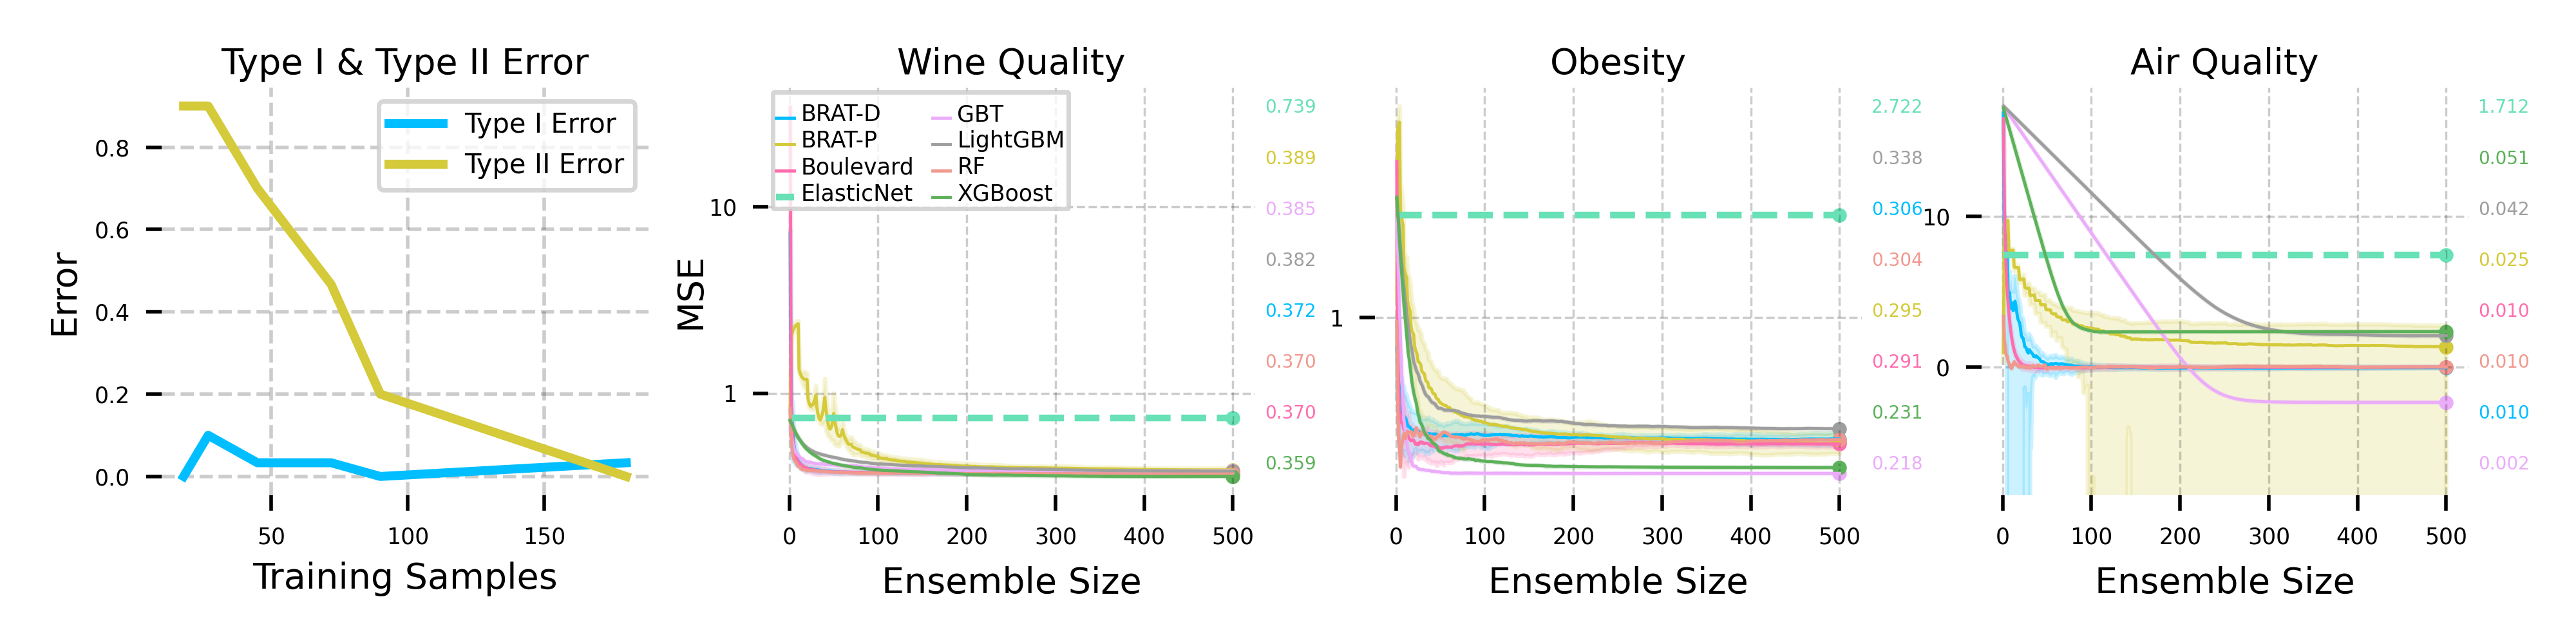
\includegraphics[width=1.1\linewidth]{figures/ch06/plots_gb/mse_tests.png}}
    \vspace{-5ex}
    \caption[Size & power / MSE races]{%
      \textbf{Left:} Type I and Type II error of the hypothesis test for variable importance against training set size. Test set is of the same size. Error rates computed over 30 trials.
      \textbf{Right:} Comparison of MSE achieved by various machine learning algorithms on different datasets, with hyperparameters tuned for each by Optuna. Shaded area depicts two standard deviations over 5 trials.
    }
    \label{fig:mse-tests}
    \vspace{1ex}
\end{figure}

% \kevin{Plot fhat over f for various K and q in order to demonstrate signal recovery}
% \kevin{Show convergence to KRR via L2 error from it}
% \kevin{Show experiments with and without integrity}


\vspace{-2ex}
\paragraph{Predictive accuracy.} The first, and most natural, thing to do is to examine the performance of our algorithms against a handful of competitors in terms of test MSE on nine datasets from the UCI Machine Learning Repository in Figure \ref{fig:mse-tests}. Our competitors include popular methods such as XGBoost \citep{chen2016xgboost}, LightGBM \citep{ke2017lightgbm}, as well as random forests and vanilla boosting. We also compare to vanilla Boulevard \citep{zhou2022boulevard}, and an elastic net regression as a baseline. All hyperparameters were tuned with Optuna \citep{optuna_2019}, reported in Appendix \ref{app:mse}. There is no clear winner in general, but XGBoost is a consistently strong performer, and random forests are clearly more suited to some datasets than others. Neither Algorithm \ref{alg:random-dropout} nor Algorithm \ref{alg:structured-dropout} consistently outperform each other, but Algorithm \ref{alg:structured-dropout} occasionally exhibits instability on some datasets. Regardless, both of our algorithms are competitive in terms of final MSE and rate of convergence, and exhibit the ability to be tuned to be closer to boosting (Wine Quality) or random forests (Air Quality), providing increased flexibility by interpolating between the two.

Our results in Figure \ref{fig:mse-tests} are somewhat unfair to Algorithm 2, as the x-axis is in the ensemble size and not the number of boosting rounds. The number of boosting rounds that Algorithm 2 encounters can be as few as 31 on Abalone, in contrast to the 500 boosting rounds all other algorithms enjoy. Given the same number of boosting rounds, we would certainly expect an improvement.


\begin{figure}[t]
    \makebox[\textwidth][c]{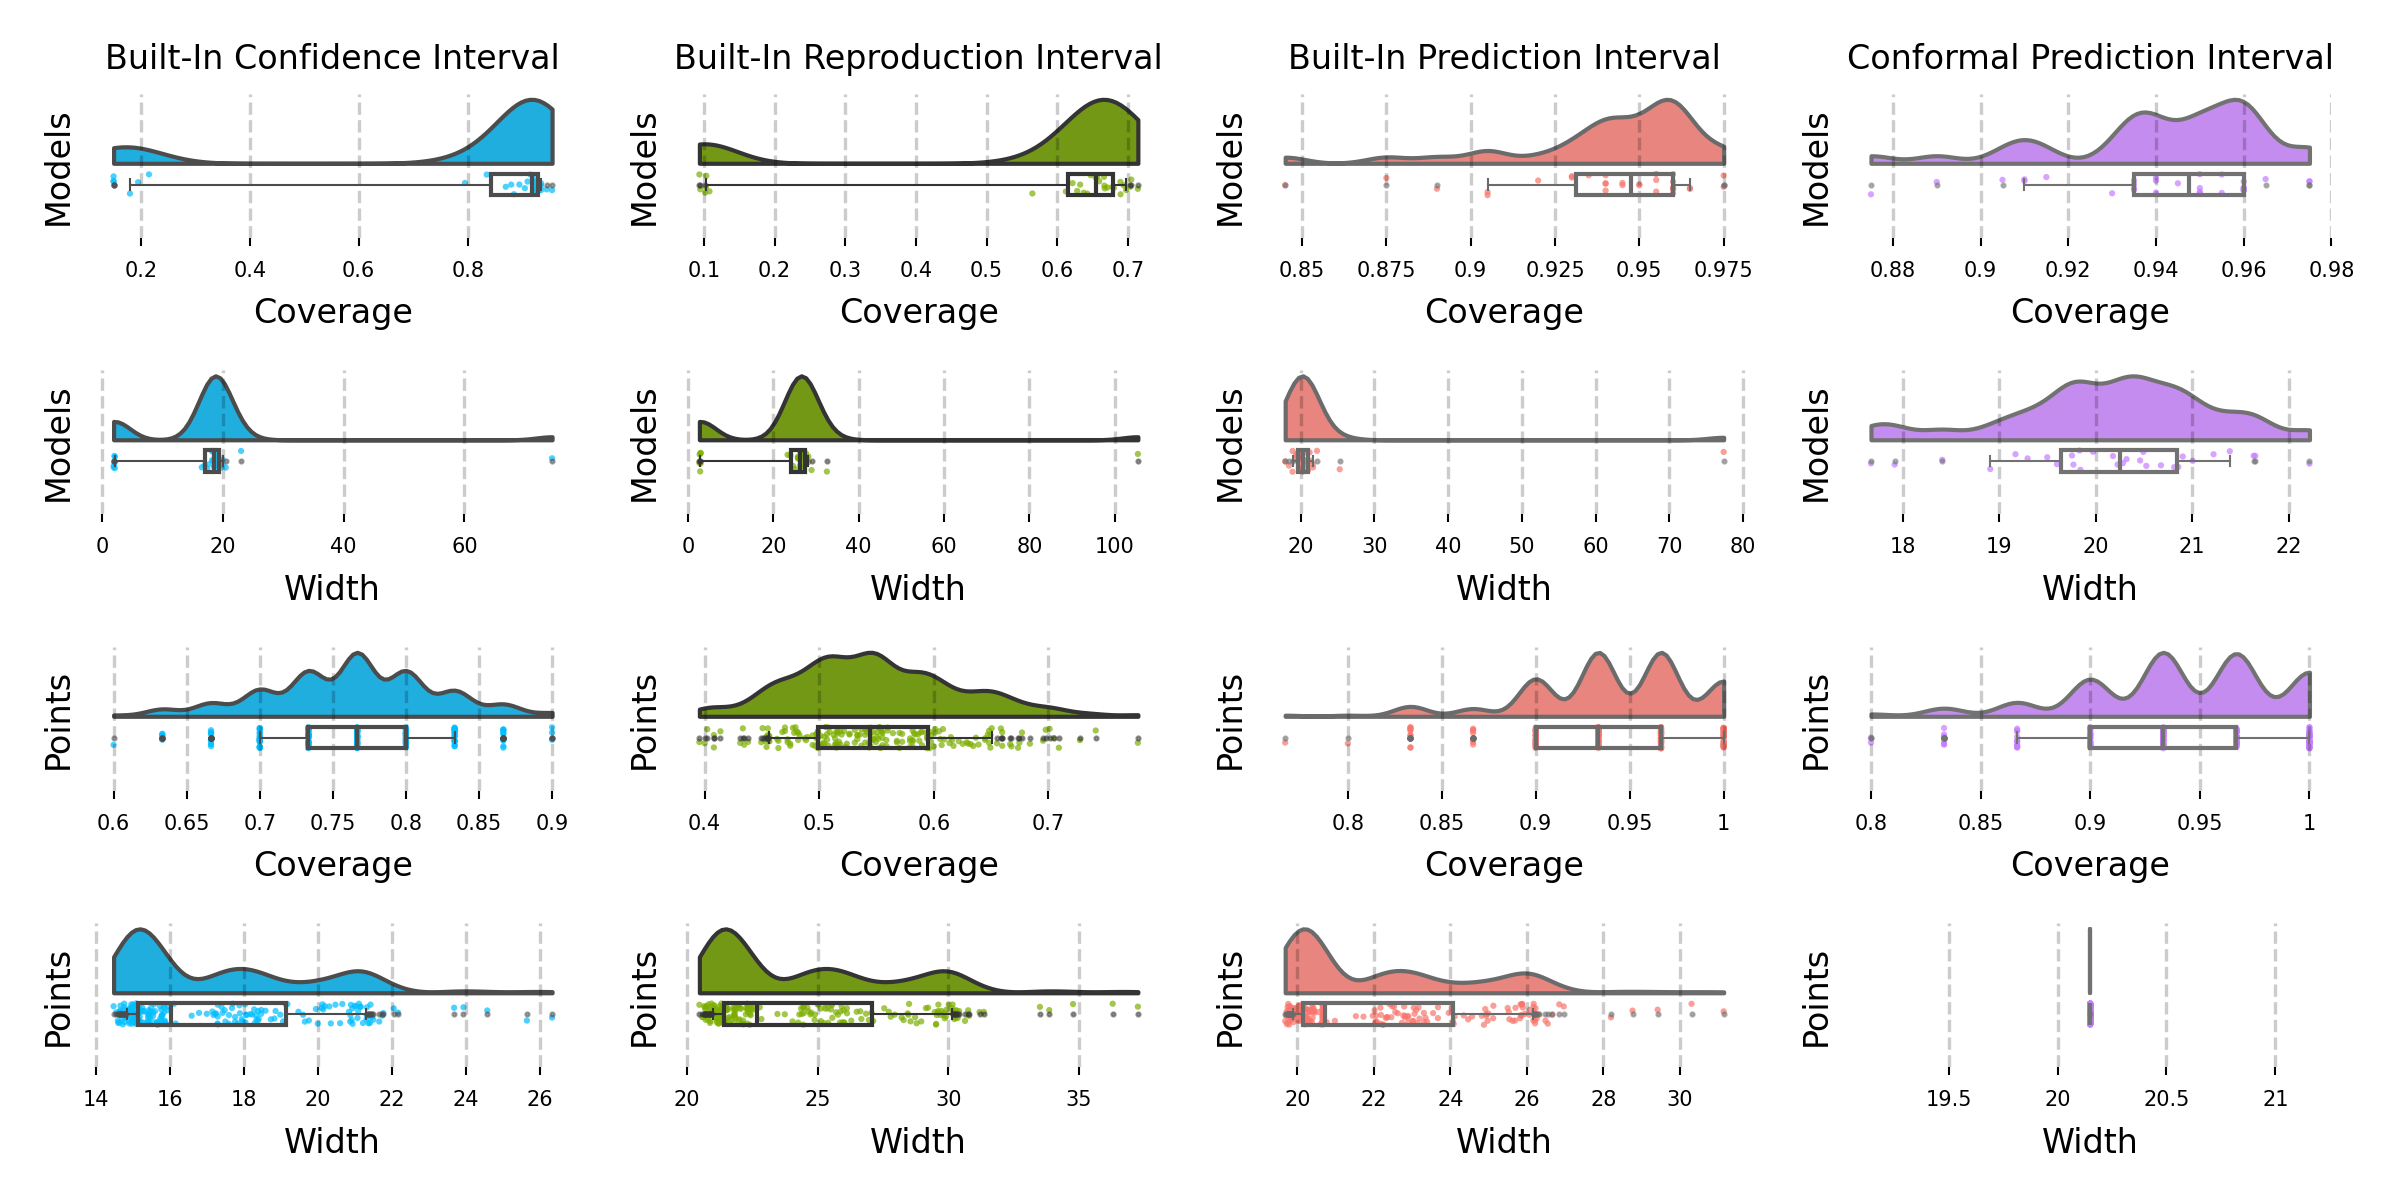
\includegraphics[width=1.1\linewidth]{figures/ch06/plots_gb/raincloud/npts_200_rep_30_epo_200_lr_0.6_sr_0.8_dr_0.3_md_4_nys_0.1_in_bag_False.png}}
    \vspace{-4ex}
    \caption{Points in the first two rows represent one of $30$ models, depicting the fraction of test points that fell inside the interval generated by the model (marginal coverage) and average width for each model. Points in the last two represent one of $100$ test points, depicting the fraction of models with intervals containing the test point (conditional coverage) and average width for each point. Results from Algorithm \ref{alg:random-dropout} with $200$ trees, learning rate $0.6$, subsampling $0.8$, dropout $0.3$, max depth $4$.}
    \label{fig:rainclouds}
\end{figure}
    
\vspace{-2ex}    
\paragraph{Variable importance tests.} We examine their performance by conducting a simulation study, testing the null $H_0:w=0$ on data from $\f(\bx)=4 x_1 -x^2_2+w bx_3$. We fit Algorithm \ref{alg:random-dropout} on data generated from $\f(\bx)$ and $\g(\bx)=4 x_1 - x^2_2$, with $100$ trees, $\lambda=1$, subsampling rate $1$, dropout rate $0.95$, and a max depth of $6$. The size and power of our test presented in Section \ref{sec:statistics} are depicted in the left panel within Figure \ref{fig:mse-tests}. Our test performs very well, maintaining appropriate size control throughout while the Type II error decreases quickly. Empirically, increasing the dropout rate increases power.
\vspace{-2ex}  
\paragraph{Coverage of intervals.}
\label{sec:coverage-experiments}
Other than the Nystr\"{o}m approximations for fast and practical interval computation in Appendix \ref{app:random-projections}, there is one more tweak that we encourage users to make in practice. We demonstrate in Corollary \ref{cor:cov-rate} that our intervals have asymptotic coverage, but this says nothing about its finite sample properties. Fortunately, \cite{candes2020adaptivecoverage} yields a simple enhancement. Since we estimate $\widehat{\sigma}$ through computing the residuals on a hold-out calibration set, we reuse the calibration set to adaptively grow or shrink our intervals according to the empirical prediction interval coverage on the calibration set. This procedure converges quickly (amounting to a doubling trick and binary search), and empirically is very helpful in increasing robustness and finite-sample performance.

To examine the empirical performance of our intervals, we consider the Friedman function $\f(\bx) = 10\sin(\pi \bx_{1}\bx_{2})+20(\bx_{3}-0.5)^{2}+5\bx_{5}-10$ \citep{friedman2000greedy}. This is depicted as a raincloud plot in Figure \ref{fig:rainclouds}. Importantly, we consider two notions of coverage: marginal coverage, where coverage is averaged over test points, and conditional coverage, where the coverage is conditional on a test point. The first two rows depict the former, while the last two depict the latter. Our intervals perform reasonably well, attaining nominal coverage with the exception of the reproduction interval's coverage and the confidence interval's conditional coverage. In particular, the prediction interval performs very well after the adaptive coverage adjustment. Importantly, unlike the conformal benchmark that has a constant width at each point, our prediction intervals have different interval widths at each point, allowing users to identify `hard'' examples. See Appendix \ref{app:rain-clouds} for other hyperparameter choices.
\vspace{-4ex}
\paragraph{CI tuning.} 
Reducing subsample rate \(\xi\) inflates variance proportionally, while deeper trees yield narrower intervals as finer splits yield sparser \(\bk_n(\bx)\) and smaller \(\|\br_n\|\).  
Variance grows with shrinkage \(1/\lambda\) and falls as dropout \(p\) increases. Choosing moderate \(\lambda\) and increasing \(p\) yields stabler CIs. Setting $p \to 0$ empirically leads to wider intervals and less power in the hypothesis test for variable importance. This can be seen in Figure \ref{fig:dropout-tests}.

%This happens as we scale Algorithm 1 by $\frac{1+\lambda (1-p)}{\lambda}$ to correct the bias. As a result, the irreducible error will be scaled up as well -- but less so when $p$ is large. A higher dropout rate also introduces decorrelation between trees, suggesting a stabler variance estimate. 

\vspace{-2ex}
\begin{figure}[H]
    \centering
    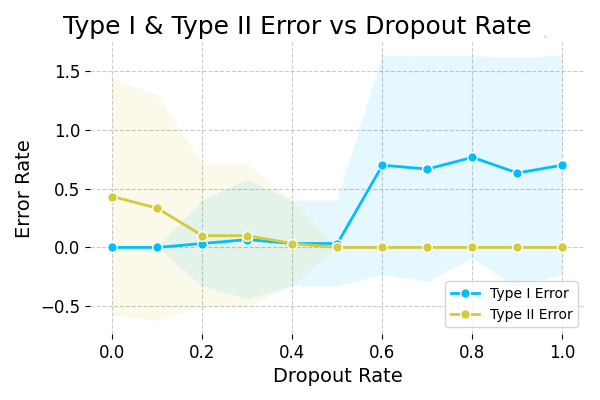
\includegraphics[width=0.49\linewidth]{figures/ch06/plots_gb/camera/size_power_dr.png}
    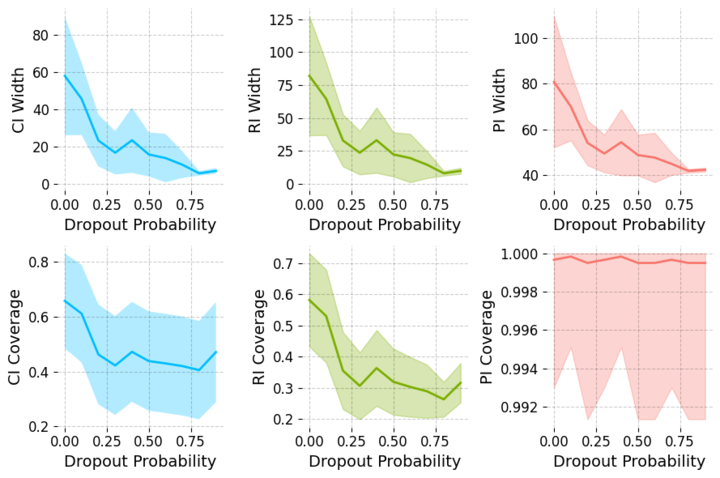
\includegraphics[width=0.49\linewidth]{figures/ch06/plots_gb/camera/ci_dropout_prob.png}
    \vspace{-1ex}
    \caption{Comparison of size and power of statistical inference procedures against dropout probability. Conformal adjustment is not performed (for clearer benchmarking, hence the under/overcovarage), and we plot the coverage and width across all datapoints and repetitions.}
    \label{fig:dropout-tests}
\end{figure}
\vspace{-2ex}

\vspace{-4ex}
\subsection{Conclusions and Further Work}
\vspace{-2ex}
\label{sec:discussions}
We incorporate dropout and parallel boosting into the regularization procedure of \cite{zhou2022boulevard}, allowing for increased signal recovery and improved asymptotic variance. With the CLTs our algorithms enjoy, we construct confidence and prediction intervals, and hypothesis tests for variable importance. Numerical experiments empirically validate our algorithms and statistical procedures.

Our theoretical guarantees depend on structure–value isolation, non‑adaptivity, and tree regularity assumptions. Relaxing these -- e.g., via honesty‐based splitting or quantifying mild adaptivity -- would broaden applicability. Extending inference beyond regression (to classification, survival, or structured outputs) also poses new challenges: non‑quadratic losses, different tree behavior, and the need for new CLTs. Doing so under weaker assumptions is a welcome direction for future work.


% \kevin{Placeholder title. There are a bunch of half-baked papers on uncertainty quantification in boosting: https://arxiv.org/pdf/2006.10562, https://arxiv.org/abs/2304.11732, and some less half baked papers like https://arxiv.org/abs/1910.03225. Ultimately previous work has neither asymptotic nor finite-sample guarantees on the coverage of any confidence intervals on the predictions generated, save for e.g. boulevard. Note that you can get a prediction interval via quantile regression, but this is not a CI. We are also interested in confidence intervals for the prediction $\widehat y$ (reproduction intervals, V-stat paper, but this term is not commonly used), not the outcome $y$. Can get intervals for $f$ in KRR world, but that's a stronger assumption (we may need this to call it statistical inference). }

% \kevin{This looks like KRR with an adaptive kernel. Can use this for a kernelized conformal prediction interval! https://jmlr.csail.mit.edu/papers/volume22/18-558/18-558.pdf but for boosting. Conformal prediction interval but we weight by in-leaf proximity. For boosting, can use same calculation we used to get the CLT to get the weights for conformal inference. }

% \kevin{So what will we have? Inference for $\widehat y$ and $f$. Provided via a few different ways, e.g. structure-value isolation (yhat and f and y as long as we can say something about the bias, i.e. need to build deep enough trees $\log n$ and analyze how large that is via the stefan wager paper (Theorem 5.3, when you scale it up it's unbiased within the existing theory, given strong assumptions made), built-in solution via KRR CIs), infinitesimal jackknife and combinations of models (only if we approx. a random forest, also just yhat, https://arxiv.org/pdf/2209.00147. Haimo says it works for f and y if depth is log n though), bootstrap (yhat and f and y, where the latter can be improved with a bootstrap bias correction, but this is the benchmark), and conformal (this can get you a prediction interval for a new draw of $y$). As well as variable importance and interactions via knockoffs (http://www.jmlr.org/papers/volume17/14-168/14-168.pdf, https://pmc.ncbi.nlm.nih.gov/articles/PMC6428414/pdf/nihms-1504775.pdf), where hypothesis testing is more needed (statistically principled variable importance)?}

% \kevin{How will we test SVI? Test coverage and width of SVI CIs against bootstrap, IJ, and conformal. }

% \kevin{How does this improve over vanilla boulevard? Vanilla boulevard converges to only half the signal, nothing more than a squashed sequential random forest. Dropout lets you recover bits of the signal so you converge to $1/(2-\rho)$ of the signal where $\rho$ is the dropout percentage. Why? When building the ensemble, even if we choose only a small percentage of trees, we still divide by the total number, oversquashing the partial ensemble and letting us recover more signal when building later trees. Hedging between current ensemble and future trees, in the sense that we think the current partial ensemble may not be right. This performs much better, and still looks like an average of trees, giving me a KRR limit to tailor. }

% \kevin{Show how to do hypothesis testing via inverting the CIs. Also perform hypothesis testing for variable importance and interactions. Can we also test for SVI? Haimo thinks it might start holding after a few trees. }

% \kevin{Would also be helpful to provide some PAC-style theory on boosting within this framework. This is just to cover our bases against a CS-style reviewer. The proofs are pretty textbook, at least for the classification case. }

% Have to assume they have 0 background information:
% 1. List all findings and position yourself. Come up with a good story. When does your algorithm work? What's missing in previous literature? 
% - Do not make it seem like it was written by Giles or Yichen. You can maybe say that Boulevard is the only algorithm with asymptotic guarantees usable for inference, but the algorithm performs poorly and 
% - We perform parallel boosting in minibatches, and incorporate dropout for regularization. The Boulevard averaging trick is used to obtain asymptotic guarantees, as it is the only one available in the literature. 
% - Write paragraph on technical difficulty/theoretical novelty in the main paper
% - Change notation, use boldface font for matrices and vectors

% 2. Experiment reasonably good: simulation + real world dataset
% (1) simulation: when your algo good and others bad (why you good, others bad)
% (2) read world: UCI repo. prediction accuracy against benchmarks 
% (3) real world: beijing housing. CI coverage plus prediction accuracy

% 3. Contributions. You need three:
% - We provide a modern boosting algorithm with built in uncertainty quantification. Produce confidence intervals, reproduction intervals, hypothesis tests, etc.
% - Our algorithm interpolates between boosting and random forests. If you set the dropout rate to 1, we recover the random forest algorithm. 
% - Extension to interpretable ML explainable boosting machines. Link between structured dropout and EBM -- apply this to EBM by boost decision stumps on each covariate to get an additive model. 

% beijing is very big. hence you can divide up the dataset in say 40. 
% break beijing up into 40 decent sized subsets, produces repetitions that you can compute coverage from
% experiments should deal with prediction accuracy as well as CI coverage

% proposal for next week. reorganize the experiment and tabulate the results.

% literatures: 




\section{Part II: Statistical Inference for Explainable Boosting Machines}
\label{sec:ch06-part2}

\begin{aigenblock}
While Part~I established pointwise asymptotic normality and sketched uncertainty quantification for general multidimensional regression trees, many scientific and high-stakes decision-making domains require interpretable generalized additive decompositions $f(\bx) = \mu + \sum_{k=1}^p f_k(x_k)$ together with componentwise confidence bands for each individual feature effect $f_k$. In Part~II, based on joint work with Haimo Fang, Jonathan Pipping, and Giles Hooker \citep{fang2026statistical}, we analyze cyclic univariate moving-average boosting (Algorithm~\ref{alg:brebm_ident}), establish finite-sample convergence to a block-structured backfitting fixed point and componentwise central limit theorems, and show that operating in histogram bin space reduces the per-query variance calculation from $O(n^3)$ to $O(M^3)$ where $M = \sum_{k=1}^p m_k \ll n$ is the total number of feature bins.
\end{aigenblock}
\subsection{Introduction}
	Modern machine learning methods have proven to be highly successful, achieving impressively high performance even for complicated prediction tasks. Still, this comes at a cost. These methods have been critiqued for their lack of transparency, often described as ``black-box'' models. As such, much work has been done in an attempt to provide explanations for their behavior.\footnote{Popular methods include LIME \cite{ribeiro2016should}, SHAP \cite{lundberg2017unified}, ALE \cite{apley2020visualizing} and partial dependence \cite{friedman2001greedy} plots.}Another line of work attempts to convince practitioners to instead use inherently transparent models that are algebraically simple enough to be inspected by humans \cite{rudin2019stop}. Neither is optimal. Explaining black-box models is a difficult problem \cite{hooker2021unrestrictedpermutationforcesextrapolation, fryer2021shapleyvaluesfeatureselection}, and inherently interpretable models can sacrifice performance. 
	
	In light of this, Explainable Boosting Machines (EBM) \cite{yin2012intelligible, nori2019interpretmlunifiedframeworkmachine} have emerged as a popular ``glass-box'' model to strike a balance between both. An EBM learns a Generalized Additive Model (GAM) \cite{hastie1986gams}: $\f(\bx) = \sum_{k=1}^{p}\f^{(k)}(\bx^{(k)})$, where each $\f^{(k)}$ is assumed to be a univariate function of the $k$-th feature. However, instead of fitting splines, it instead fits a set of univariate gradient boosting regression trees. The tree-based boosting procedure attempts to recover the expressiveness of state-of-the-art algorithms \cite{chen2016xgboost, ke2017lightgbm}, while the decomposition into additive components allows the measurement of the marginal contribution of each feature like linear models.  While EBMs impose strong structural constraints on the resulting prediction, their ability to reproduce nonlinearities, along with appropriate choices of additive structure, provides comparable performance to SOTA boosting \cite{nori2019interpretmlunifiedframeworkmachine}. 
	
	
	\begin{figure*}[ht!]
    \vspace{-2ex}
		\centering
		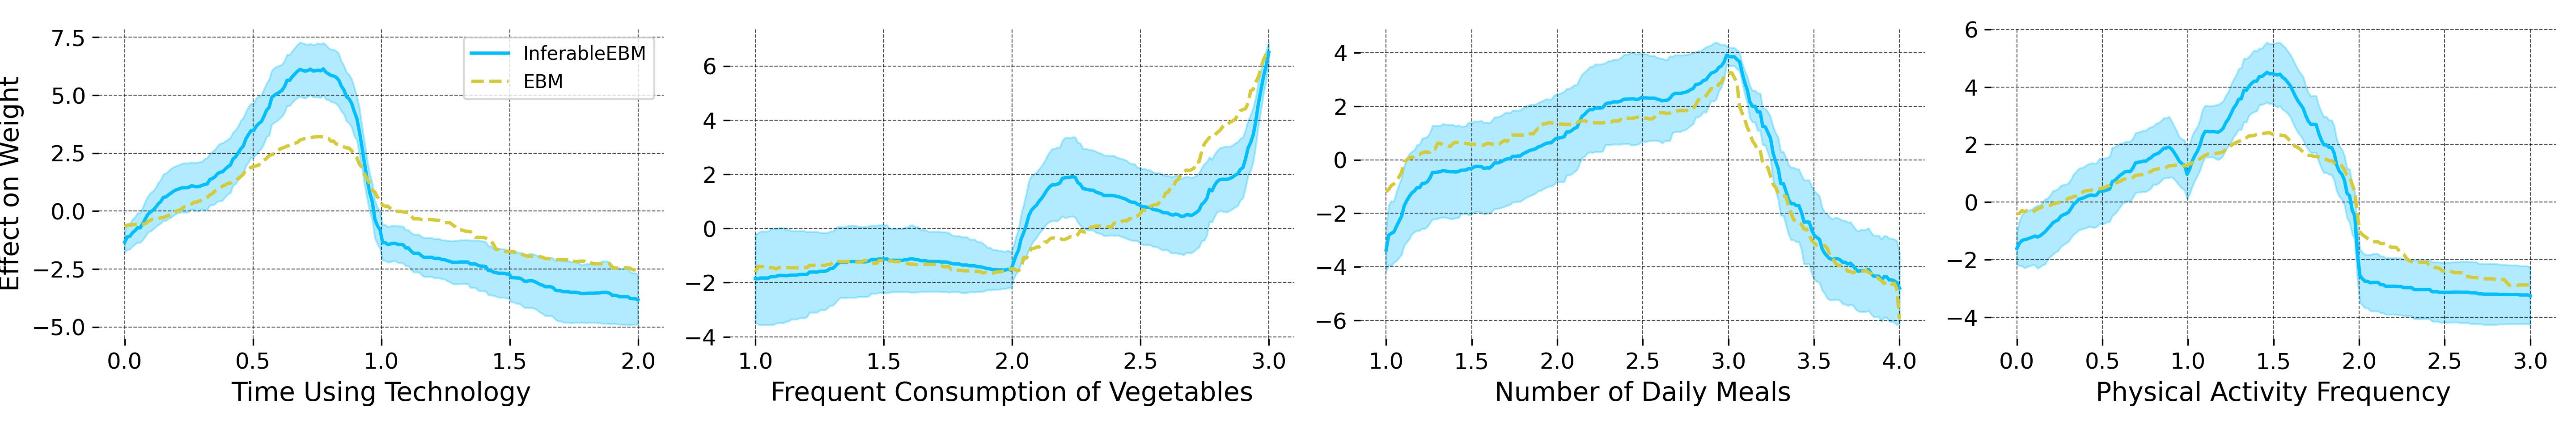
\includegraphics[width=\linewidth]{figures/ch06/plots_ebm/obesity_feature_effects_wide.png}
		\vspace{-4ex}
		\caption{Example of the feature-specific confidence intervals generated by Algorithm \ref{alg:brebm_ident}, compared to the point estimates from EBM \cite{nori2019interpretmlunifiedframeworkmachine}. This visualizes centered feature effects on the UCI Machine Learning Reposity Obesity \cite{estimation_of_obesity_levels_based_on_eating_habits_and_physical_condition__544} dataset, when predicting weight as the response. }
		\label{fig:ebm-effects-wide}
        \vspace{-2ex}
	\end{figure*}
	
	While EBMs provide a clear graphical representation for the effects of each feature, these are still point estimates. The central question we ask for uncertainty quantification can be phrased as this: \textit{Given a model design, if we collect a new dataset and retrain the model, how different would our new prediction be?} In response to this question, vanilla EBMs \cite{yin2012intelligible} compute variance estimates via bootstrapping, though this is computationally intensive and only heuristically justified. Our primary objective is hence \emph{well-calibrated frequentist uncertainty quantification} for EBMs while retaining their interpretability and scalability.

	
	A canonical alternative to bootstrapping is to construct confidence and prediction intervals using the asymptotic properties of the model. This is the case with GAMs fitted via the backfitting (but not boosting) algorithm, which enjoy a rich asymptotic theory that enables the construction of confidence and prediction intervals for them \cite{2f43af29-e27b-3b6f-9c3a-d7c3bd53adac}. Another widely used alternative for prediction intervals is conformal prediction, which provides finite-sample marginal coverage with minimal assumptions. However, conformal methods do not directly yield feature-wise confidence intervals for the GAM components, which we aim to explore in this work.
	
	Unfortunately, the asymptotic behavior of most gradient boosting algorithms (of which EBMs are one), is not known. \cite{ustimenko2023gradientboostingperformsgaussian} show that a randomized version of boosting converges to a Gaussian process. On the other hand, \cite{zhou2019boulevardregularizedstochasticgradient} show that taking an average instead of a sum of trees (in a process which they call Boulevard regularization) converges to a kernel ridge regression, yielding asymptotic normality. This was recently leveraged by \cite{fang2025gradient} to construct confidence intervals for the underlying nonparametric function $\f$ and prediction intervals for the labels, with extensions to random dropout and parallel boosting.

    \paragraph{Our contributions.}
     Unfortunately, the underlying nonparametric function itself can be highly complicated and uninterpretable in general. Restricting this to the class of GAMs, as with EBMs, yields interpretability. However, the existing Boulevard theory \cite{zhou2019boulevardregularizedstochasticgradient} does not directly apply to the class of algorithms we consider here. These results need to be extended to allow different structure matrices (resulting in different kernels) for each feature, along with enforcing the GAM identifiability conditions. While we sketch an algorithm that can be analyzed largely within the framework of \cite{fang2025gradient}, further algorithmic variants that either employ backfitting directly or employ parallelization methods result in different algorithmic limits requiring separate analysis. Unlike prior Boulevard analyses, EBMs induce \emph{feature-specific} kernels. This makes the theory substantially more delicate: one must control their interaction under centering and GAM identifiability, and establish asymptotic normality for each additive component, not just the overall predictor. To handle these additional challenges, we make the following contributions:
     
	\vspace{-2ex}
	\begin{itemize}
		\item \textbf{Asymptotic Theory.} We establish central limit theorems for three variations of EBMs (parallelized, backfitting-like parallelized, and sequential), showing that the Boulevard-regularized ensemble converges to a feature-wise kernel ridge regression. The resulting predictions are asymptotically normal and achieve the minimax-optimal MSE of $O(pn^{-2/3})$ for fitting Lipschitz $p$-dimensional GAMs \cite{yuan2015minimaxoptimalratesestimation}. This avoids the curse of dimensionality, significantly improving upon the rates of \cite{zhou2019boulevardregularizedstochasticgradient, fang2025gradient}.
		
		\item \textbf{Frequentist Inference.} By leveraging our proposed CLT for baseline vector $\bbeta$ and feature-wise predictions $\widehat \f^{(k)}$, we extend the heuristic bootstrap to a set of inference toolkits. We provide confidence intervals for each underlying function $\f^{(k)}$ (see Figure \ref{fig:ebm-effects-wide} for an example), and prediction intervals for the response. This also allows a direct test of variable importance following the methods of \cite{mentch2015quantifyinguncertaintyrandomforests}. We round out those propositions by numerical experiments to back up the validity of our algorithms.
		
		\item \textbf{Computational Efficiency.} The derived procedures above rely on a kernel ridge regression, with a prohibitively expensive $O(n^3)$ runtime. \cite{fang2025gradient} employ the Nyström approximation to produce intervals in $O(np^2)$ kernel precomputation and $O(p^2)$ query time, but the recursive implementation of \cite{musco2017recursivesamplingnystrommethod} can be slow in practice. Given that EBMs utilize histogram trees, we instead work out the computations in histogram bin-space.
        This bin-based implementation runs in an additional lower-order $O(pm^2)$ time per training round, $O(pm^3)$ kernel precomputation time, and $O(pm^2)$ interval query time, where $p$ is the number of features and $m$ the maximum number of bins per-feature. As the number of bins is usually capped at $255$ or $511$, this is independent of the number of samples $n$!
	\end{itemize}
	\begin{figure*}[ht!]
    \vspace{-3ex}
    \centering
     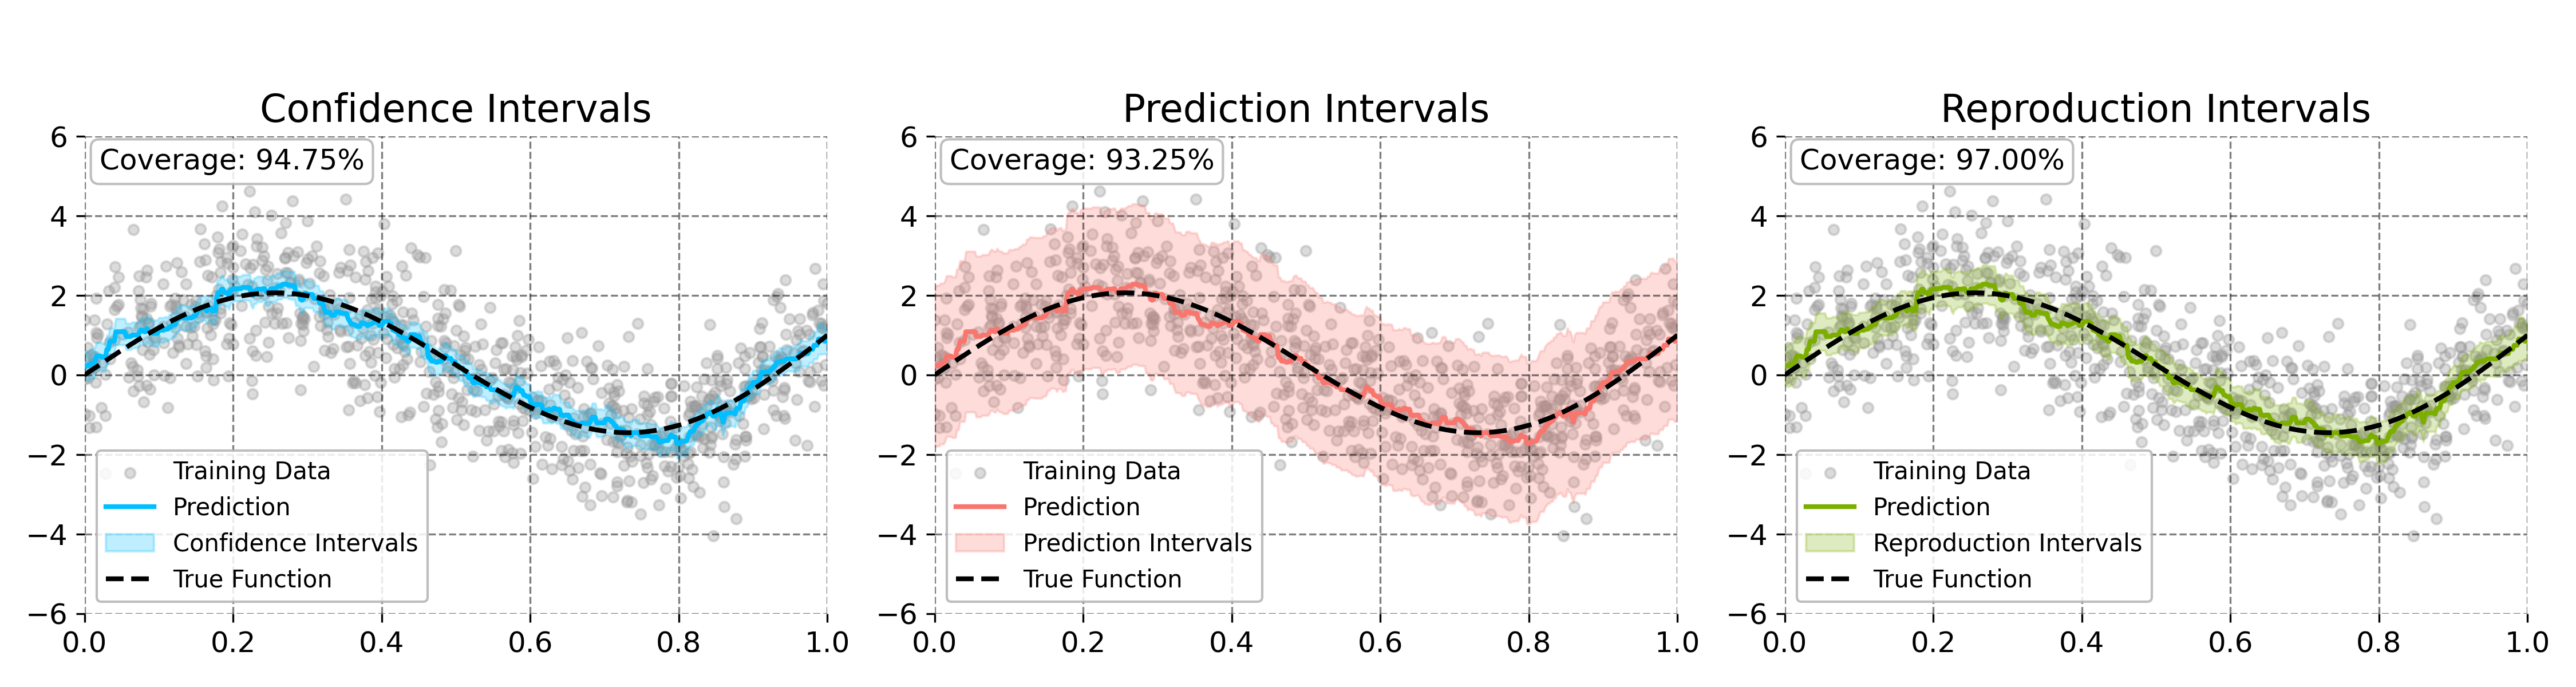
\includegraphics[width=0.8\linewidth]{figures/ch06/plots_ebm/coverage_1d_plot.png}
        \vspace{-2ex}
	    \caption{Example of confidence and prediction intervals on a simple 1D function $y=2\sin(2\pi x) + x^2$.}
	    \label{fig:coverage-1d} \vspace{-2ex}
	\end{figure*}
	
	% {\bf exploitation of basis representation?}
	
	% {\bf need to sketch out results and simulations}
	\subsection{Setup and Notation}
	\label{ch06b:sec:setup}
	
	%    \kevin{Introduce plot on overfitting, and refer the reader to Fig 2 of our last paper for evidence that Boulevard avoids overfitting and allows the user to ignore the need for early stopping. The figure we will provide (overfit\_mse.png) shows that the EBM and InferableEBM frameworks are robust to this. EBM does so through a really small learning rate and random split sampling, we do so via Boulevard regularization. }
	
	Let $(\bX_n, \by_n) = (\bx_i,y_i)_{i=1}^n$ are i.i.d.\ samples with $\bx_i=(\bx_i^{(1)},\ldots,\bx_i^{(p)})^\top$. Let $\jmat=\bI_n-\frac{1}{n}\bone\bone^\top$ denote the centering projector. We adopt the standard GAM identifiability convention that each component is centered on the training set: $\sum_{i=1}^n \f^{(k)}(\bx_i^{(k)})=0$ for all $k$, so the intercept equals the sample mean. Then:
	\begin{assumption}[Additive Lipschitz Nonparametric Regression]
		\label{aspt:truth}
		Assume that the response satisfies
		$$
		y \;=\; \bbeta \;+\; \sum_{k=1}^p \mathbf{f}^{(k)}(\mathbf{x}^{(k)}) \;+\; \epsilon : = \f(\bx) + \epsilon,
		$$
		where $y, \bbeta \in\mathbb{R}$, $\mathbf{x}=(\bx^{(1)},\dots,\bx^{(p)})^\top\in\mathbb{R}^p$, and $\varepsilon$ are i.i.d.\ sub–Gaussian errors with mean zero and variance $\sigma^2<\infty$.  
		Assume the covariates have a bounded density on their support: $0<c_1\leq \mu(\mathbf{x}) \leq c_2<\infty$.  Each component function $\f^{(k)}:\mathbb{R}\to\mathbb{R}$ is mean–zero with respect to the marginal of $\bx^{(k)}$, and is $L$-Lipschitz. The intercept $\bbeta$ is defined as the unconditional mean of the response: $\bbeta := \E_{\bx, \epsilon}[y] = \int y \, d\mu_{\bx}(x)\, d\mu_\epsilon(\epsilon).$
	\end{assumption}
	
	\paragraph{Boulevard Regularization.}\cite{zhou2019boulevardregularizedstochasticgradient} replace the usual additive update with a moving average. Instead of adding the next tree: $\widehat{\f}_b \leftarrow \f_{b-1}+\lambda\bt_b$, they average over all previous trees: $\widehat{\f}_b \leftarrow \frac{b-1}{b}\f_{b-1}+\frac{\lambda}{b}\bt_b$. This idea of shrinking the previous ensemble as also been adopted by \cite{ustimenko2022sglbstochasticgradientlangevin, ustimenko2023gradientboostingperformsgaussian}. This ensures convergence to a kernel ridge regression in the limit of infinite boosting rounds, and that the resulting predictions are asymptotically normal.\footnote{A particular advantage of Boulevard regularization is that it is robust to overfitting \cite{fang2025gradient}. Figure \ref{fig:overfit_mse} shows this behavior for Algorithm \ref{alg:brebm_ident}. EBM achieves this here via tiny learning rates when cycling through features in sequence. We do this while fitting to features in parallel.}
    
	
	


	\subsection{Algorithms} \label{ch06b:sec:algorithms}
    
	\begin{algorithm}[ht!]
		\caption{\aigen{Cyclic Univariate Moving-Average Boosting for Generalized Additive Models}}
		\label{alg:brebm_ident}
		\begin{algorithmic}[1]
			\State \textbf{Input:} $\mathbf{X}\in\mathbb{R}^{n\times p}$, $\mathbf{y}\in\mathbb{R}^n$, subsample rate $\xi$, learning rate $\lambda$, rounds $B$, truncation level $M>0$.
			\State \textbf{Init:} $\widehat{\bbeta}_0 \gets \frac{1}{n}\sum_{i=1}^n \by_i$;\quad $\f_k^{(0)} \gets 0$ for all $k$.
			\For{$b=1$ \textbf{ to } $B$}
			\For{$k=1$ \textbf{ to } $p$ \textbf{ in parallel}}
			\State Sample $G_{b,k}\subset\{1,\dots,n\}$ i.i.d. w.p. $\xi$.
			\State $r_{i,k} \gets \by_i - (\widehat{\bbeta}_{b-1} + \sum_{\ell} \f_{b-1}^{(\ell)}(\bx_i^{(\ell)}))$.
			\State Fit tree $\bt^{(b,k)}$ to $\{(\bx_i^{(k)}, r_{i,k})\}_{i\in G_{b,k}}$.
			\State $\mu_{b,k} \gets \frac{1}{n}\sum_{i=1}^n \bt^{(b,k)}(\bx_i^{(k)})$.
			\State $\widetilde \bt_b^{(k)}(\bx) \gets t_b^{(k)}(\bx) - \mu_{b,k}$.
			\State $\widetilde \bt_b^{(k)}(x) \gets \max\{-M,\;\min\{\widetilde \bt_b^{(k)}(\bx),M\}\}$.
			\State $\widehat{\bbeta}_b \gets \widehat{\bbeta}_{b-1} + \mu_{b,k}$.
			\State $\f_b^{(k)} \gets \frac{b-1}{b} \f_{b-1}^{(k)} + \frac{\lambda}{b}\,\widetilde \bt_b^{(k)}$.
			\EndFor
			\EndFor
			\State \textbf{Output:} $\widehat \f(x) \gets \widehat{\bbeta}_B + \frac{1+\lambda}{\lambda}\sum_{k=1}^p \f_k^{(B)}(\bx^{(k)})$.
		\end{algorithmic}
	\end{algorithm}
	
	
    We adapt the above regularized boosting procedure to fitting EBMs below in Algorithm \ref{alg:brebm_ident}, in the hope that doing so allows us to show similar theoretical guarantees for the resulting procedure. 
    
    \paragraph{Parallelization and  inference.} Algorithm \ref{alg:brebm_ident} is a minimal parallelized variation on EBMs. At each round $b$, the new set of $p$ univariate trees $(\bt_b^{(k)})_{k=1}^p$ are fitted in parallel by regressing the current residual $r_{i,k}$ on each of the $p$ features $\bx_i^{(k)}$. The trees are then centered and clipped, before being introduced into the ensemble as part of the average: $\mathbf{f}_b^{(k)} \gets \frac{b-1}{b} \mathbf{f}_{b-1}^{(k)}+\frac{1}{b} \widetilde{\mathbf{t}}_b^{(k)}$.
    
    Averaging yields a kernel ridge regression limit and a CLT, but (as in Boulevard) the fitted signal is asymptotically shrunk, requiring rescaling by $\frac{1+\lambda}{\lambda}$. In Section \ref{sec:finite-sample-convergence}, we show that the prediction made by Algorithm \ref{alg:brebm_ident} converge to a kernel-ridge-regression. Informally:
	$$
	\widehat{\f}_b(\bx) \underset{b\to\infty}{\overset{a.s.}{\longrightarrow}} \bar{\by}+ \sum_{k=1}^{p}\E[\sveck(\bx)]^\top \jmat[\bI + \jmat\bK]^{-1}\by.
	$$
	The down-scaling stems from the matrix $[\bI + \jmat\bK]^{-1}$: When the aggregated kernel $\bK = \sum_{k=1}^{p} \Kmatk$ becomes nearly the identity (i.e. the aggregated decision boundaries are fine enough), we see a $\frac{\lambda}{1+\lambda}$ shrinkage.

    \paragraph{Difficulty in parallelization.} 
    The parallelization in Algorithm \ref{alg:brebm_ident} does not come for free. One has to either use a small learning rate of $1/p$, or make a rather strong assumption on the feature kernels (see Assumption \ref{aspt:proj-orth}) for Algorithm \ref{alg:brebm_ident} to provably converge.
    
    Though in practice this is not an issue, we explore alternatives below for the sake of completeness. One is to abandon parallelism, and randomly choose a single feature to fit a tree to during each boosting round. This is presented in Algorithm \ref{alg:brebm_random_cyclic} (see Appendix \ref{ch06b:app:algorithms}), which converges to the same fixed point as Algorithm \ref{alg:brebm_ident}, but without the computational gains. 
	
	\paragraph{Leave-one-out procedure.} One problem remains. Algorithms \ref{alg:brebm_ident} and \ref{alg:brebm_random_cyclic} converges to $\frac{\lambda}{1+\lambda} \f \leq \f/2$, and so require rescaling by $\frac{1+\lambda}{\lambda}$. 
    We provide an alternative inspired by the backfitting-like procedure of \cite{fang2025gradient} in Algorithm \ref{alg:ebm_bratp} that does not require rescaling. 
    
    This hybrid backfitting-boosting procedure amounts to not using predictions from trees trained on feature $\bx^{(k)}$ when fitting a new tree $\bt_{b}^{(k)}$ for it\footnote{This can be interpreted as treating other functions $\f^{(\ell)} \neq \f^{(k)}$ as nuisances and learning them via boosting, while learning $\f^{(k)}$ as a random forest.} -- instead using  residuals $\by_i - (\widehat{\bbeta}_b+\sum_{\ell\neq k}\f_{b-1}^{(\ell)}(\bx_i^{(\ell)}))$.
    Although this does not require rescaling, it produces complicated confidence intervals that are harder to compute efficiently. Informally, Algorithm \ref{alg:ebm_bratp} converges to:
	$$
	\bar{\by}+ \sum_{k=1}^{p}\E[\sveck(\bx)]^\top (\bI - \E\Smatk)^{-1} \jmat\Big[\bI-(\bI+\mathcal{K})^{-1}\mathcal{K}\Big]\by,
	$$
    where $\mathcal{K}:=\sum_{k=1}^p(\mathbf{I}-\mathbb{E} \mathbf{S}^{(k)})^{-1} \mathbf{J}_n \mathbb{E} \mathbf{S}^{(k)}$ is a somewhat more complicated combined kernel that unlike Algorithms \ref{alg:brebm_ident} and \ref{alg:brebm_random_cyclic}, does not decompose into the sum of the individual feature kernels. 
	\paragraph{Comparison to vanilla EBMs.} Our algorithms possess advantages over vanilla EBMs. The convergence to a kernel ridge regression allows us to show a central limit theorem for each function $\f^{(k)}$:
    $$\lVert\rveck(\bx)\rVert_2^{-1}\left(c_E\cdot\widehat{\f}^{(k)}(\bx) - \f^{(k)}(\bx)\right)\stackrel{d}{\longrightarrow}\mathcal{N}(0, \sigma^2),$$
    where $c_E$ is a scaling factor that is $\frac{\lambda}{1+\lambda}$ for Algorithms \ref{alg:brebm_ident} and \ref{alg:brebm_random_cyclic}, and $1$ for Algorithm \ref{alg:ebm_bratp}. $\rveck$ are the kernel weights for the kernel ridge regression predictions ${\rveck}^\top\by$. For instance, Algorithms \ref{alg:brebm_ident} and \ref{alg:brebm_random_cyclic} converge to ${\rveck}^\top\by := \mathbb{E}\left[\mathbf{s}^{(k)}(\mathbf{x})\right]^{\top} \mathbf{J}_n\left[\mathbf{I}+\mathbf{J}_n \mathbf{K}\right]^{-1} \by.$
    
    This asymptotic normality yields confidence intervals for each $\f^{(k)}$ and prediction intervals for the response $\by$ -- as long as we can compute $\lVert\rveck(\bx)\rVert_2$ efficiently. It also allows us to prove guarantees on the generalization error of each algorithm. We later show that $\lVert\rveck(\bx)\rVert_2 = \Theta(n^{-1/3})$, allowing us to show that our algorithms achieve the minimax-optimal MSE of $O(p\,n^{-2/3})$ for fitting Lipschitz GAMs. In comparison, vanilla EBMs hold \emph{no such guarantees}.
    
    % By incorporating Boulevard regularization, one replace the heuristic error band with asymptotic variance $\sigma_{\widehat{\f}}^2 = \norm{\rveck}\sigma^2$, where $\rveck$ is the kernel-ridge-regression style operator we introduce later in section \ref{ch06b:sec:theory}. Following the same intuition in \cite{zhou2019boulevardregularizedstochasticgradient}, the ultimate prediction is down-scaled by $\frac{\lambda}{1+\lambda}$. As a complement, Algorithm \ref{alg:ebm_bratp} is proposed to avoid such scaling.

    \paragraph{Comparison to Boulevard.} The original gradient boosting algorithm with Boulevard regularization of \cite{zhou2019boulevardregularizedstochasticgradient} converges to a kernel ridge regression of the form $\E[\bs(\bx)]^\top(\lambda^{-1}\bI + \E[\bS])^{-1}\E[\bS]\by$. This is similar to our result for Algorithms \ref{alg:brebm_ident} and \ref{alg:brebm_random_cyclic}, but we achieve convergence for each centered univariate function while they achieve convergence only for the overall function $\f$. As a consequence, their method has an MSE of $O(n^{-\frac{1}{d+1}})$ that grows exponentially in dimension. This is not even minimax-optimal for the nonparametric Lipschitz regression setting they are in.
    
    The variants of \cite{fang2025gradient} incorporating dropout and parallel training converge to slightly different fixed points, but ultimately achieve the same asymptotic MSE rates exponential in dimension.
    
    % By way of comparison, in standard Boulevard trees have access to all features at once. \cite{fang2025gradient} added a dropout mechanism to the method first described in \cite{zhou2019boulevardregularizedstochasticgradient} in which trees are fit to residuals obtained after randomly dropping $(1-q)\%$ of the current ensemble resulting in a limit given by 
    % $\E \mathbf{s}(\bx) ^T (\lambda^{-1}\bI + q \E \Smat)^{-1} \E \Smat \by$
    % for a single expected tree structure matrix $\E \Smat$ which is approximately downscaled by $\lambda/(1+\lambda q)$.  A structured dropout algorithm that effectively divided the ensemble into $K$ groups, but with the same distribution over structure matrices, obtained a limit of $\E \mathbf{s}(\bx)^T(I + (K-1)\E \Smat)^{-1} K \E \Smat \by$, obviating the need to rescale. The analysis of this limit is simpler in comparison to those given above in having a common structure matrix and removing the identifiability concerns that motivate recentering. 
    
%    \kevin{Compare fixed points with Boulevard fixed points.}
	
    \subsection{Theory}
    \label{ch06b:sec:theory}
    We now work towards proving the central limit theorem outlined above. To begin, we introduce a few definitions. First, we use regression trees as base learners. These can be understood as a linear transformation from the observed signal to the predictions via a smoothing tree kernel, formally defined below:
	\begin{definition}[Regression trees]
		\label{def:regression-trees}
		A regression tree $\bt_n$ trained on $n$ datapoints segments the covariate space $[0,1]^d$ into a partition of hyper-rectangles $\{A_i\}_{i=1}^m$. When $A(\bx)$ is the rectangle containing $\bx$, and $s_{n,j}(\bx)$ is the frequency at which training point $\bx_j$ and test point $\bx$ share a leaf, ${s}_{n,j}(\bx) = \frac{\mathbbm{1}(\bx_j \in A(\bx))}{\sum_{k=1}^n \mathbbm{1}(\bx_k \in A(\bx))},$ the regression tree $\bt_n$ predicts $\bt_n(\bx) = \sum_{j=1}^n s_{n,j}(\bx)\cdot y_j$.
	\end{definition}
	This suggests that ${s}_{n,j}(\bx)$, the frequency at which training point $\bx_j$ and test point $\bx$ share a leaf, defines a similarity measure. This observation is insightful. In fact, the frequency at which training points $\bx_i, \bx_j$ share a leaf, $s_{n,j}(\bx_i)$, yields a kernel!\footnote{Theorem 3 of \cite{zhou2019boulevardregularizedstochasticgradient} shows that $\E\bS_n$ is p.s.d. with spectral norm no more than 1.}
	\begin{definition}[Structure vectors and matrices]
		\label{def:structure-vec-mat}
		Let $\bt_n$ be a tree. $\bs_n(\bx) = (s_{n,1}(\bx),...,s_{n,n}(\bx))^\top$ be the structure vector of $\bx$. The matrix $\bS_n = \left(s_{n,j}(\bx_i)\right)_{i,j=1}^n$ with rows $\bs_n(\bx_i)^\top$ is the structure matrix of $\bt_n$.
	\end{definition}
	Following \cite{zhou2019boulevardregularizedstochasticgradient, fang2025gradient}, we require that the tree \emph{structures} be separated from the leaf  \emph{values}, and stabilize after a burn-in period:
	\begin{assumption}[Integrity]
		\label{aspt:integrity}
		Assume
        \vspace{-2ex}
		\begin{enumerate}
			\item (Structure-Value Isolation) The density for $\bs_b(\bx)$ is independent from the terminal leaf value $\by\in\mathbb{R}$.
			\item (Non-adaptivity) For each feature $k$, there exists a set of probability measures $\mathcal{Q}^{(k)}_n$ for tree structures such that all tree structures $\Smatk_b$ are independent draws from $\mathcal{Q}^{(k)}_n$ after some finite $b'$.
		\end{enumerate}
	\end{assumption}
	
	The former can be satisfied by refitting leaf values on a hold-out dataset \cite{wager2017estimationinferenceheterogeneoustreatment}. Non-adaptivity may occur naturally, but can also be enforced by sampling from previous tree structures after a burn-in period. In practice, our algorithms tend to perform well even in the absence of these assumptions.
	
	\paragraph{Tree Geometry}
	We control the geometry and size of leaves to ensure locality and stable averages. These assumptions control the MSE of the final estimate -- \cite{zhou2019boulevardregularizedstochasticgradient} and \cite{fang2025gradient} make spiritually similar assumptions, but with  different scalings in dimension that do not avoid the curse of dimensionality. Again, we avoid this problem due to the GAM structure of our problem setup:
	\begin{assumption}[Bounded Leaf Diameter]
		\label{ch06b:aspt:leaf-diameter}
		Write $\mathsf{diam}(A)=\sup_{\bx_1,\bx_2\in A}\norm{\bx_1-\bx_2}$. For any leaf $A$ in a tree with structure $\Pi\in Q_n^{(k)}, \forall k = 1, \cdots, p$, we need $\sup_{A \in \Pi} \mathsf{diam}(A) =  O(d_n) = O(n^{-{1}/{3}})=o(\frac{1}{\log n})$.
	\end{assumption}
    Assumption \ref{ch06b:aspt:ub-minimal-leaf-size} forces trees to perform only \emph{local} averaging by keeping leaves well-balanced. Assumption \ref{aspt:truth} allows depths as large as $\Omega(\log n)$, which is natural for balanced binary trees.
	
	\vspace{-1ex}
	\begin{assumption}[Increased Minimal Leaf Size]
		\label{ch06b:aspt:ub-minimal-leaf-size}
		For any $\nu >0$, the leaf geometric volume $v_n$ is bounded such that \(v_n =n^{-\frac{2}{3}+\nu}<n^{-\frac{1}{3}}=O(d_n)\).
	\end{assumption}

    This is natural: the leaf count cannot exceed the effective histogram resolution. Enforcing at least $n^{2/3-\nu}$ points per leaf rules out overly fine, high-variance partitions.

    
	\begin{assumption}[Restricted Tree Support]
		\label{ch06b:aspt:restricted-tree-space}
		For a tree constructed using feature $k$, the cardinality of the tree space $Q_n^{(k)}$ is bounded by $O\Big(n^{-1/3}\exp(n^{2/3-\epsilon_n})\Big)$, for some small $\epsilon_n \to 0$.
	\end{assumption}

    This is a technically convenient assumption for us to generalize it in random design case. It bounds the effective complexity of the tree class so we can use uniform LLNs and contraction arguments. The assumption still permits an super-polynomial large class in $n$, which is far looser than practice: vanilla EBMs use very shallow trees (typically depth 1--2) on a fixed histogram grid with at most a few hundred bins per feature, so the effective class is much smaller (roughly polynomial in $n$).
    
	Unlike \cite{zhou2019boulevardregularizedstochasticgradient} and \cite{fang2025gradient}, the assumptions above are dimension-free. They enforce asymptotic locality of the partition, allowing for control over bias and variance. Assumption \ref{ch06b:aspt:ub-minimal-leaf-size} ensures stability of the structure matrix spectrum, allowing us to recover the minimax-optimal rate later.

    \paragraph{Warmup: Theory for Algorithm 
    \ref{alg:brebm_random_cyclic}.}

    
    As mentioned earlier, the theory for Algorithm \ref{alg:brebm_random_cyclic} is  the easiest to prove. With the following observation, this amounts to a straightforward extension of \cite{zhou2019boulevardregularizedstochasticgradient}. The learner updates a feature's kernel at random each round, so the tree kernel chosen by Algorithm \ref{alg:brebm_random_cyclic} amounts to $\E\bS = \frac{1}{p}\sum_{k=1}^p\E[\Smatk]$. 
    
    This observation allows us to apply the theory of \cite{zhou2019boulevardregularizedstochasticgradient} almost verbatim. As such, Algorithm \ref{alg:brebm_random_cyclic} gives a spiritually similar fixed point iteration $\tilde{\by}^*:=\sum_{k}\hat{\by}_k^*=\lambda\jmat\E\bS(\by - \tilde{\by}^*)$\footnote{We drop intercepts as they are orthogonal to centering.}, modulo centering. This leads to a ensemble-wise fixed point of $\tilde{\by}^* = (\bI + \jmat\E\bS)^{-1}\jmat\E\bS\by$ and the subsequent feature-wise fixed points $\hat{\by}_k^* = \lambda\jmat\E\bS(\bI - (\bI + \jmat\E\bS)^{-1}\jmat\E\bS)\by=\lambda\jmat\E\Smatk(\bI + \jmat\E\bS)^{-1}\by$. Finite sample convergence and asymptotic normality holds following the same recipe discussed in \cite{zhou2019boulevardregularizedstochasticgradient}.

    However, this sequential random update does not parallelize over features. 
    To address these concerns we return to  Algorithm \ref{alg:brebm_ident} and analyze its convergence, which we will discuss in Section \ref{subsec:alg.1}.

    \paragraph{Feature-specific (specialized) kernels.}
	Still, the above intuition is instructive. Unlike \citet{zhou2019boulevardregularizedstochasticgradient} and \citet{fang2025gradient}, which consider a single expected kernel $\E\bS$, EBMs induce \emph{feature-specific} kernels $\Kmatk:=\E[\Smatk]$.  This is a double-edged sword. On one hand, one has to control the way these kernels interact in our algorithms. On the other, it enables a clearer characterization of partial dependence, while allowing us to demonstrate feature-wise convergence, which in turn yields feature-wise confidence intervals. 

    \paragraph{Theory for Algorithm \ref{alg:brebm_ident}.}
    \label{subsec:alg.1}
    
    As mentioned earlier in Section \ref{ch06b:sec:algorithms}, introducing parallelization introduces theoretical challenges. One way to prove that Algorithm \ref{alg:brebm_ident} converges is to use a learning rate of $\lambda =\frac{1}{p}$. However, this yields no speedup from Algorithm \ref{alg:brebm_random_cyclic} on average, as sampling with probability $1/p$ and averaging across $p$ updates are the same in expectation. 

    Another way, that allows us to use a learning rate of $\lambda \approx 1$, is to make the following assumption:
    
	\begin{assumption}[Projector-like feature kernels and conditional orthogonality]
		\label{aspt:proj-orth}
		Let $\Kmatk=\E[\Smatk]$ and $\jmat:=\bI_n-\frac{1}{n}\bone\bone^\top$. 
		For each feature $k$, let
		$$
		\mathcal H_k \;:=\; \big\{\,\bv\in\R^n:\ \exists\,g:\R\!\to\!\R\text, \bv_i=g(\bx_i^{(k)}),\ \bone^\top \bv=0\,\big\}
		$$
		with $P_k$ the orthogonal projector onto $\mathcal{H}_k$. Assume:
		\begin{itemize}
			\item \textbf{Projector-like approximation.} There exists $\varepsilon_{n,k}\to 0$ with
			$\big\|\, \jmat\,\Kmatk\,\jmat - P_k \,\big\|_{\mathrm{op}} \;\le\; \varepsilon_{n,k}\,.
			$
			\item \textbf{Conditional orthogonality.} For $a\neq k$, the additive subspaces are orthogonal:
			$
			P_a\,P_k \;=\; \mathbf{0}\,.
			$
		\end{itemize}
	\end{assumption}
	Assumption~\ref{aspt:proj-orth} is technically convenient but admittedly strong, especially the conditional orthogonality requirement. We therefore emphasize that it is used only to analyze Algorithm~\ref{alg:brebm_ident}. As a fallback, Algorithm~\ref{alg:ebm_bratp} removes this requirement and needs only Assumption~\ref{aspt:kernel-spec}. Intuitively, the projector-like condition says the centered expected tree kernel for feature $k$ behaves like the orthogonal projector onto mean-zero functions of $\bx^{(k)}$, while conditional orthogonality asserts these per-feature subspaces have negligible overlap across $k$ (similar in spirit to “no concurvity” conditions for uniqueness in additive models, e.g., \citealp{hastie1986gams}); this can hold exactly under feature independence and can be a reasonable approximation under weak dependence when partitions are shallow and not aligned across features.
    

    
    Now we discuss the finite-sample convergence for Algorithm \ref{alg:brebm_ident} as promised. A way forward is to first establish almost surely convergence as we keep boosting with $b\to \infty$, then seek asymptotic normality when sample size grows. The first part is usually handled by showing that the difference to a set of postulated fixed points is a stochastic contraction mapping, decaying to 0. However, by the design of Algorithm \ref{alg:brebm_ident}, stepwise mean convergence can be fragile when $\lambda \approx 1$, hence we enforce Assumption \ref{aspt:proj-orth} to ensure stability. Formally, the convergence behavior can be characterized in Theorem \ref{thm:finite-sample-convergence-1}, stated below.
    
    \begin{theorem}
		\label{thm:finite-sample-convergence-1}
		Define $\widehat{\mathbf{y}}_{b}:=\widehat{\bbeta}_{b}+\sum_{a=1}^{p}\widehat{\mathbf{y}}^{(a)}_{b},
		\jmat=\bI-\tfrac{1}{n}\bone\bone^\top.$
		The fixed points are
		\[
		\widetilde{\mathbf{y}}_k^* \;=\; \jmat\,\Kmatk\,[\lambda^{-1}\bI+\jmat\,\bK]^{-1}\mathbf{y},
		\qquad
        \bK\;:=\;\sum_{k=1}^{p}\Kmatk,
        \]
		and $\widehat{\mathbf{y}}^*\;=\;\widehat{\bbeta}^*\bone+\sum_{k=1}^{p}\widetilde{\mathbf{y}}_k^*$,
		with $\widehat{\bbeta}^*=\bar{\mathbf{y}}$. For each $k$,
        $$
        \widehat{\mathbf{y}}^{(k)}_{b}\;\stackrel{a.s.}{\longrightarrow}\; \widetilde{\mathbf{y}}^{(k)\,*},
		\qquad
		\widehat{\bbeta}_{b}\;\stackrel{a.s.}{\longrightarrow}\;\bar{\mathbf{y}}=\tfrac{1}{n}\bone^\top\mathbf{y},
		$$
		and hence $\widehat{\mathbf{y}}_{b}\stackrel{a.s.}{\to} \widehat{\mathbf{y}}^*$ almost surely.
	\end{theorem}

    This fixed point carries two different relevant and practical perspectives. When setting $\lambda = \frac{1}{p}$, one essentially implements a coordinate descent. It also recovers the vanilla boulevard randomized tree kernel by assigning uniform mass on featurewise kernels. Thus convergence can be shown without additional assumptions. Taking $\lambda=1$, however, requires a more delicate characterization of tree behavior specified in Assumption \ref{aspt:proj-orth}. This condition implies that featurewise signals do not overlap with each other asymptotically, removing the need for averaging the final feature functions.\footnote{This can be thought of as parallel coordinate descent. Averaging is conservative, so when can we not do so?}

    \paragraph{Theory for Algorithm \ref{alg:ebm_bratp}.}
    As discussed before, one may argue that Assumption \ref{aspt:proj-orth} is unrealistic. If one is not willing to use $\lambda=1/p$ then, Algorithm \ref{alg:ebm_bratp} poses a remedy. This does not rely on Assumption \ref{aspt:proj-orth}, and only depends on a weaker assumption below.
    \begin{assumption}[Feature-kernel distinctness]
		\label{aspt:kernel-spec}
		Let $\Kmatk=\E[\Smatk]$. There exists $c_3<1$ such that, for all $a\ne k$,
			$
			\big\|\, \E[\mathbf{S}^{(a)}]\,\E[\Smatk] \,\big\|_{\mathrm{op}} \;\le\; c_3,
			\quad
			(p-1)\,c_3 \;<\; 1.
			$
	\end{assumption}
	
    Assumption~\ref{aspt:kernel-spec} is a weaker version of Assumption~\ref{aspt:proj-orth}: instead of requiring (approximate) orthogonality of feature-wise subspaces, it only rules out the degenerate case where different features induce nearly identical smoothing operators in expectation. We verified this assumption empirically with plausible results. See Table \ref{tab:kernel_distinctness}. This milder assumption is sufficient for establishing a similar finite-sample convergence result below.


    \begin{theorem}
		\label{thm:finite-sample-convergence-2}
		Denote the prediction using feature $k$ at boosting round $b$ as $\widehat{\mathbf{y}}^{(k)}_b = \frac{1}{b}\sum_{s=1}^bt^{(s, k)}(\mathbf{x}^{(k)})$.
		Define the aggregated kernel $\mathcal{K}:=\sum_{k=1}^{p}(\bI-\E\Smatk)^{-1}\jmat\E\Smatk$. Define feature-wise fixed points
		\[
		\widetilde{\mathbf{y}}_k^* = (\bI-\E\Smatk)^{-1} \jmat\E\Smatk\left[\bI - \left(I+\mathcal{K}\right)^{-1}\mathcal{K}\right]\mathbf{y}.
		\]
		Then, $\widehat{\mathbf{y}}^{(k)}_b \overset{a.s.}{\to}\widetilde{\mathbf{y}}_k^*$, $\widehat{\mathbf{y}}_b\overset{a.s.}{\to}\widehat{\mathbf{y}}^*$, and $\widehat{\bbeta}^* \overset{a.s.}{\to}\bar{\mathbf{y}}:=\frac{1}{n}\mathbf{1}^\top\mathbf{y}.$
		
	\end{theorem}

    The operator $(\bI-\Smatk)^{-1} (\bI-\frac{1}{n}\mathbf{1}\mathbf{1}^\top)\Smatk$, which we can interpret as a feature-wise KRR, is stacked with the fixed point of the residual created on the whole ensemble. In this product, $(\bI-\Smatk)^{-1} (\bI-\frac{1}{n}\mathbf{1}\mathbf{1}^\top)\Smatk$ measures the marginal contribution of a particular feature $k$ contribute to the ensemble prediction. 

    \paragraph{A Central Limit Theorem.} We are now in a position to provide central limit theorems for all three algorithms. Unlike \cite{zhou2019boulevardregularizedstochasticgradient} and \cite{fang2025gradient}, the GAM structure of our problem allows us to relax the rates within the assumptions on tree geometries. While the following lemma allows us to check the Lindeberg-Feller conditions, it also allows us to recover the optimal minimax rate $n^{-2/3}$ for univariate non-parametric Lipschitz regression \cite{yuan2015minimaxoptimalratesestimation}. Below, we use the subscript $E=\{A,B\}$ to label relevant variables in Algorithm \ref{alg:brebm_ident} and \ref{alg:ebm_bratp}. 

    \begin{lemma}[Rate of Convergence]
		\label{ch06b:lem:rateofr}
		Let $\mathbf{B}^{(k)}_n := \{i  : \norm{\bx^{(k)}-\bx_i^{(k)}}\leq d_n\}$ be the points within distance $d_n$ from test point $\bx$ on feature $k$. Under Assumption \ref{ch06b:aspt:restricted-tree-space}, if $\left| \mathbf{B}_n \right|  = \Omega( n \, d_n)$ and $\inf_{A\in \Pi\in Q_n^{(k)}}\sum_{i}\bI(\bx_i\in A) = \Omega(n^{\frac{2}{3}})$, then
		$
		\norm{\kveck}_2,
		\norm{\rveck_E}_2 = \Theta(n^{-\frac{1}{3}})
		$ almost surely.
	\end{lemma}

	The rate of the boulevard vector enables a conditional CLT, informally $\frac{\rveck_E(\bx)^\top\f(\bX)-\f^{(k)}(\bx)}{\norm{\rveck_E(\bx)}}\overset{d}{\to}\mathcal{N}(0, \sigma^2)$. Working with either Assumption \ref{aspt:proj-orth} or Assumption \ref{aspt:kernel-spec}, we analyze the form of the combined kernel, and conclude with the following central limit theorem.

    \begin{theorem}[Asymptotic Normality]
		\label{thm:unconditional-clt}
		Define $c_A = \frac{\lambda}{1+\lambda}, c_B=1 $. For all $k = 1, \cdots, p$, we have that:
		$$\norm{\rveck_E(\bx)}^{-1}\left(\widehat{\f}_E^{(k)}(\bx)-c_E\f^{(k)}(\bx)\right) \overset{d}{\rightarrow} \mathcal{N}(0, \sigma^2)
		$$
	\end{theorem}

    Normality of the intercept term $\hat{\bbeta}$ is also established and discussed in Lemma \ref{thm:baseline-clt}. Similar to \cite{fang2025gradient}, our CLTs yields a subsequent risk bound:
    \begin{corollary}
    \label{cor:risk-bound}
        $\E[(\frac{1}{c_E}\hat{\f}_E^{(k)}(\bx)-\f^{(k)}(\bx))^2] \lesssim \frac{\sigma^2}{c_E^2}p\,n^{-\frac{2}{3}}$.
    \end{corollary}
    This result shows that our algorithms achieve the minimax-optimal MSE of $O(pn^{-2/3})$ for fitting Lipschitz $p$-dimensional GAMs \cite{yuan2015minimaxoptimalratesestimation}. This avoids the curse of dimensionality, significantly improving upon the rates of \cite{zhou2019boulevardregularizedstochasticgradient, fang2025gradient}.

    \begin{figure*}[ht!]
     \vspace{-2ex}\centering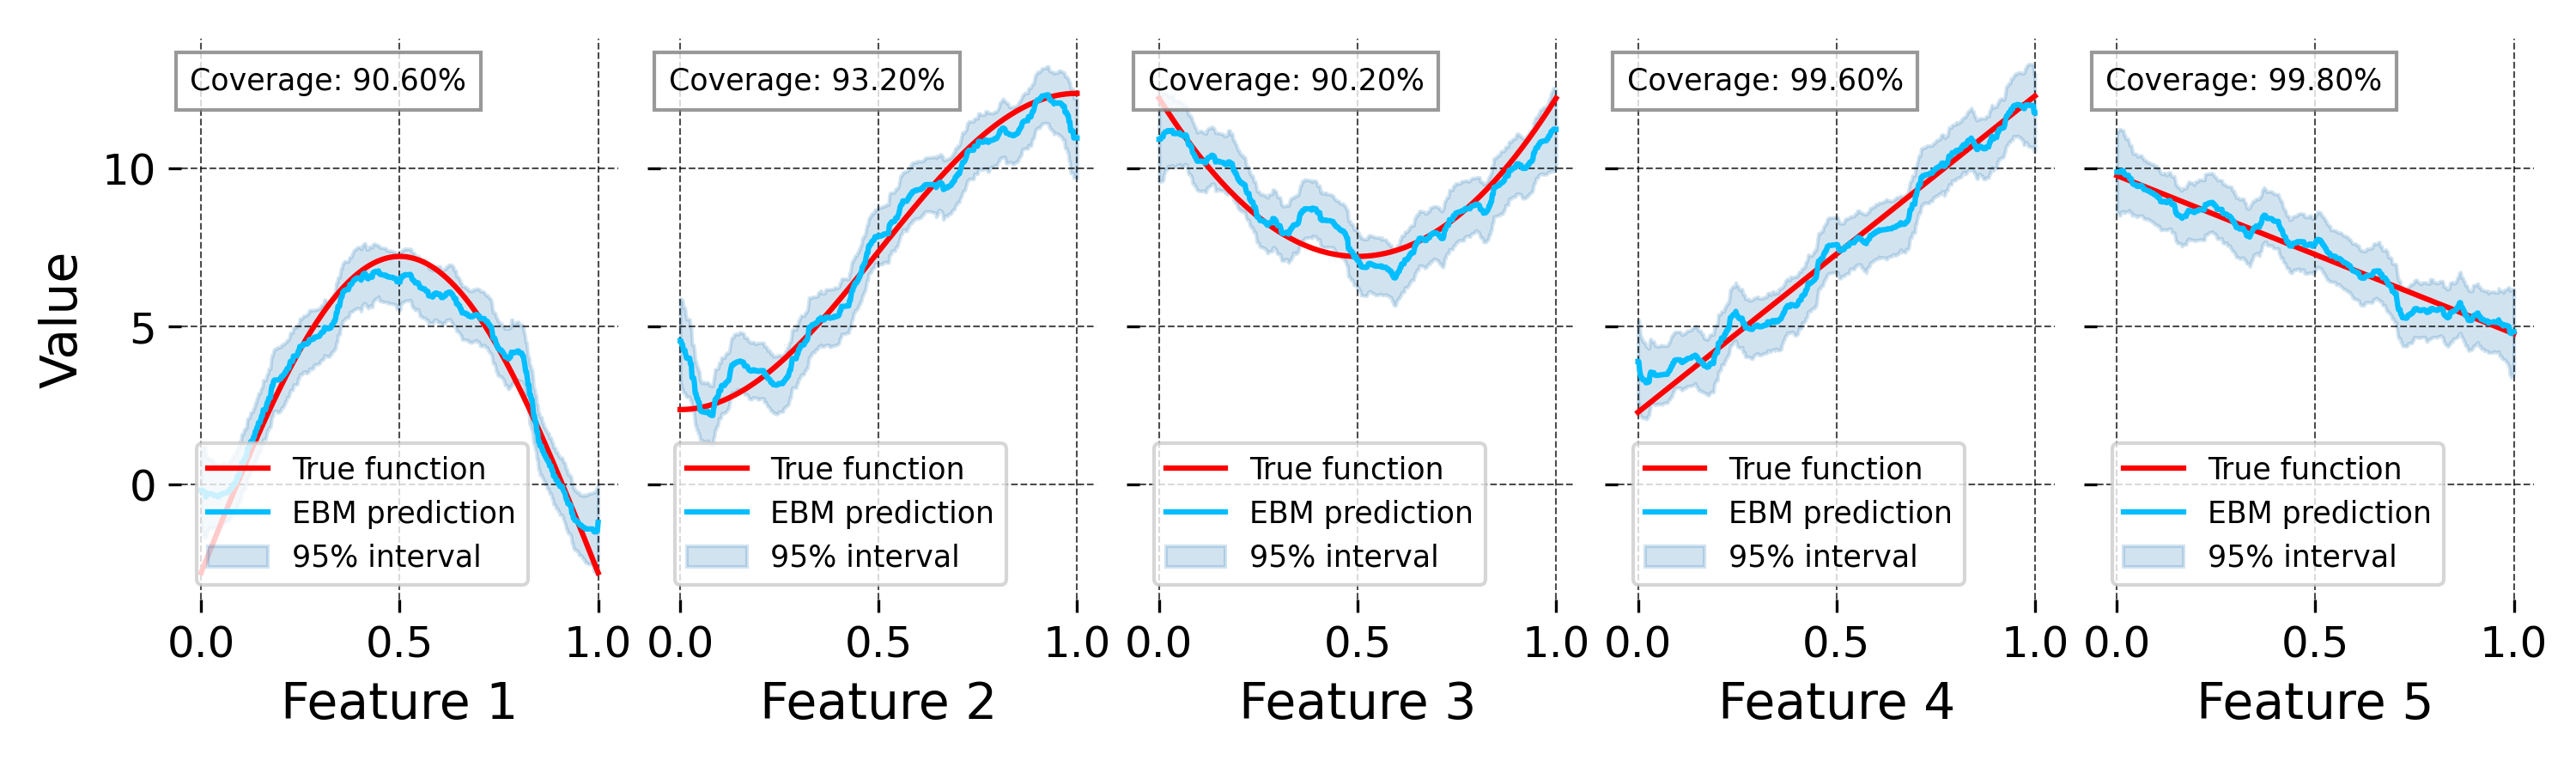
\includegraphics[width=0.7\linewidth]{figures/ch06/plots_ebm/feature_interval_plots.png}\vspace{-2ex}
        \caption{Per-feature CIs and coverages for $f(x)=-5+10\sin(\pi x^{(1)}) + 5\cos(\pi x^{(2)}) + 20(x^{(2)}-0.5)^2  +10x^{(3)} - 5x^{(4)}$.}
        \label{fig:feature-coverage}
        \vspace{-2ex}
    \end{figure*}

    % \begin{corollary}[PAC Guarantee]
    % \label{cor:pac-updated}
    % If $n \;\ge\; C_1\!\left\{\Big(\tfrac{L}{\varepsilon}\Big)^{\!3}\;\vee\;\Big(\tfrac{\sigma^2\log(2/\delta)}{\varepsilon^2}\Big)^{\!\!3/2}\right\}$ and $b \;\ge\; C_2\;\frac{\lambda^2 M^2\, n^{1/3}}{\varepsilon^2\,\delta},$ then with probability at least $1-\delta$,
    % \(
    % \big|\hat f^{(b)}_n(x)-f(x)\big|\le \varepsilon.
    % \)
    % \end{corollary}
    
	\subsection{Inference and Computation}
    We can now derive confidence and prediction intervals from the result on asymptotic normality above. Here, we construct practical intervals and tests, and shows how to compute the required standard errors in \emph{bin space} so that inference time is independent of $n$. Throughout the section, we estimate the noise variance with a consistent variance estimates $\hat{\sigma}^2$ via in-sample or out-of-bag estimation.

    
    \paragraph{Confidence Intervals.}
    We construct $(1-\alpha)$ confidence intervals for each of \{individual feature effects, the intercept, the values of a prediction at a new $\bx$\}.
    \vspace{-2ex}
    \begin{itemize}
        \item $c_E^{-1}\widehat{\f}^{(k)}_E(\bx)\ \pm\ z_{1-\alpha/2}\,c_E^{-1}\hat{\sigma}\,\lVert\rveck_E(\bx)\rVert$ yields a $(1-\alpha)$-confidence interval for the feature effect. By similar arguments in \cite{fang2025gradient}, the coverage rate will converge to $(1-\alpha)$ almost surely. This is validated by an example in Figure  \ref{fig:feature-coverage}.
        \item For the intercept term, by Lemma~\ref{thm:baseline-clt}, $\widehat{\bbeta}$ is asymptotically normal with variance $\sigma^2/n$, yielding the usual interval $\widehat{\bbeta}\pm z_{1-\alpha/2}\,\hat{\sigma}/\sqrt{n}$
        \item For the overall response, write $\widehat{f}_E(\bx)=\widehat{\bbeta}+c_E^{-1}\sum_{k=1}^p \widehat{\f}^{(k)}_E(\bx)$. A $(1-\alpha)$ confidence interval is
    $\widehat{f}_E(\bx)\ \pm\ z_{1-\alpha/2}c_E^{-1}\hat{\sigma}\sqrt{\frac{1}{n}+\|\sum_{k=1}^p \rveck_E(\bx)\|_2^2\ }.
    $
    \end{itemize}
    \vspace{-2ex}
    Recall that $\rveck_E(\bx)$ denotes the per-feature influence vector. Under Assumption~\ref{aspt:proj-orth}, $\lVert\sum_{k=1}^p \rveck_E(\bx)\rVert_2^2
    =\sum_{k=1}^p \lVert{\rveck_E(\bx)}\rVert_2^2,$ so the variance contribution is the sum of feature-wise terms. Without Assumption~\ref{aspt:proj-orth}, this replacement is conservative by Cauchy–Schwarz.

    \cite{fang2025gradient} examines two further variants that are immediately implementable:
    \vspace{-1ex}
    \begin{itemize}
    \item {\bf Reproduction Intervals.} All intervals above can be modified to be {\em reproduction} intervals for the predictions of a new model trained on an independent dataset by scaling their widths by $\sqrt{2}$. %\cite[see][]{zhou2019boulevardregularizedstochasticgradient}. This has the interpretation that 
    %they cover a replication of the estimate on new data with probability $(1-\alpha)$. 

%    To get reproduction intervals, scale the bandwidth of CIs by $\sqrt{2}$. The subsequent intercept intervals and response intervals can be constructed as shown in the previous paragraph.


 %   \paragraph{Prediction and Reproduction Intervals} 
 %   As discussed by \cite{fang2025gradient}, we can construct the prediction intervals and reproduction intervals for featurewise predictions and intercepts, with almost sure convergence of coverage rates. 
    
    \item {\bf Prediction Intervals.} We can construct  a prediction interval for a new $y$ given $\bx$ by computing ${c_E}^{-1}{\widehat{\f}^{(k)}_E(\bx)}\ \pm\ z_{1-\alpha/2}\,{c_E}^{-1}{\hat{\sigma}\sqrt{1+\lVert{\rveck_E(\bx)}\rVert_2^2}}$. 
\end{itemize}

    \paragraph{Binning. } The current implementation of EBMs \cite{nori2019interpretmlunifiedframeworkmachine} utilizes histogram trees. As we worked off this implementation, it was natural to construct intervals with the binned data, instead of working with the original data. A more detailed discussion of the discretization error induced by binning is deferred to Appendix~\ref{append:what_we_lose_by_binning}.
    
    As such, we compress all $n$ samples along feature $k$ into $m_k\!\ll\!n$ histogram bins and work entirely in \emph{bin space}. In Appendix~\ref{app:binning}, we construct a decomposition of the structure matrix that allows us to show that computing the norm of $\rveck(\bx)$ reduces to solving a $m_k\times m_k$ system of linear equations, and computing two $m_k$-length dot products. 
    
    After this compression, the dependence on $n$ disappears. Denote $m$ as the maximum number of bins among all $k$ binnings. Caching $\bM$ takes $O(pm^3)$, while each per-point inference query takes only $O(m^2)$ time. As bin numbers are often capped to 255 or 511 (independent of $n$), we can compute our intervals in time independent of the number of samples. This outperforms \cite{fang2025gradient}'s runtime of $O(nd_{\text{eff}}^2)$.

    \paragraph{Practical Guidance.} In practice, Algorithm \ref{alg:brebm_ident} relies on conditional orthogonality; we recommend monitoring simple convergence diagnostics, and if convergence appears unstable, falling back to Algorithm \ref{alg:ebm_bratp}. In our experiments, the number of boosting rounds $B$ in the range 100--300 worked well. A smaller learning rate $\lambda$ typically improves finite-sample stability but can yield slightly wider intervals. Subsample rates in $[0.5,0.8]$ were robust. For binning, we found that using either the usual EBM defaults (e.g., 64 or 255 bins) or scaling the bin count as $m\asymp n^{1/3}$ works well; the latter matches our assumptions.

    \addtocounter{figure}{1}
    \begin{figure*}[ht!]
        \centering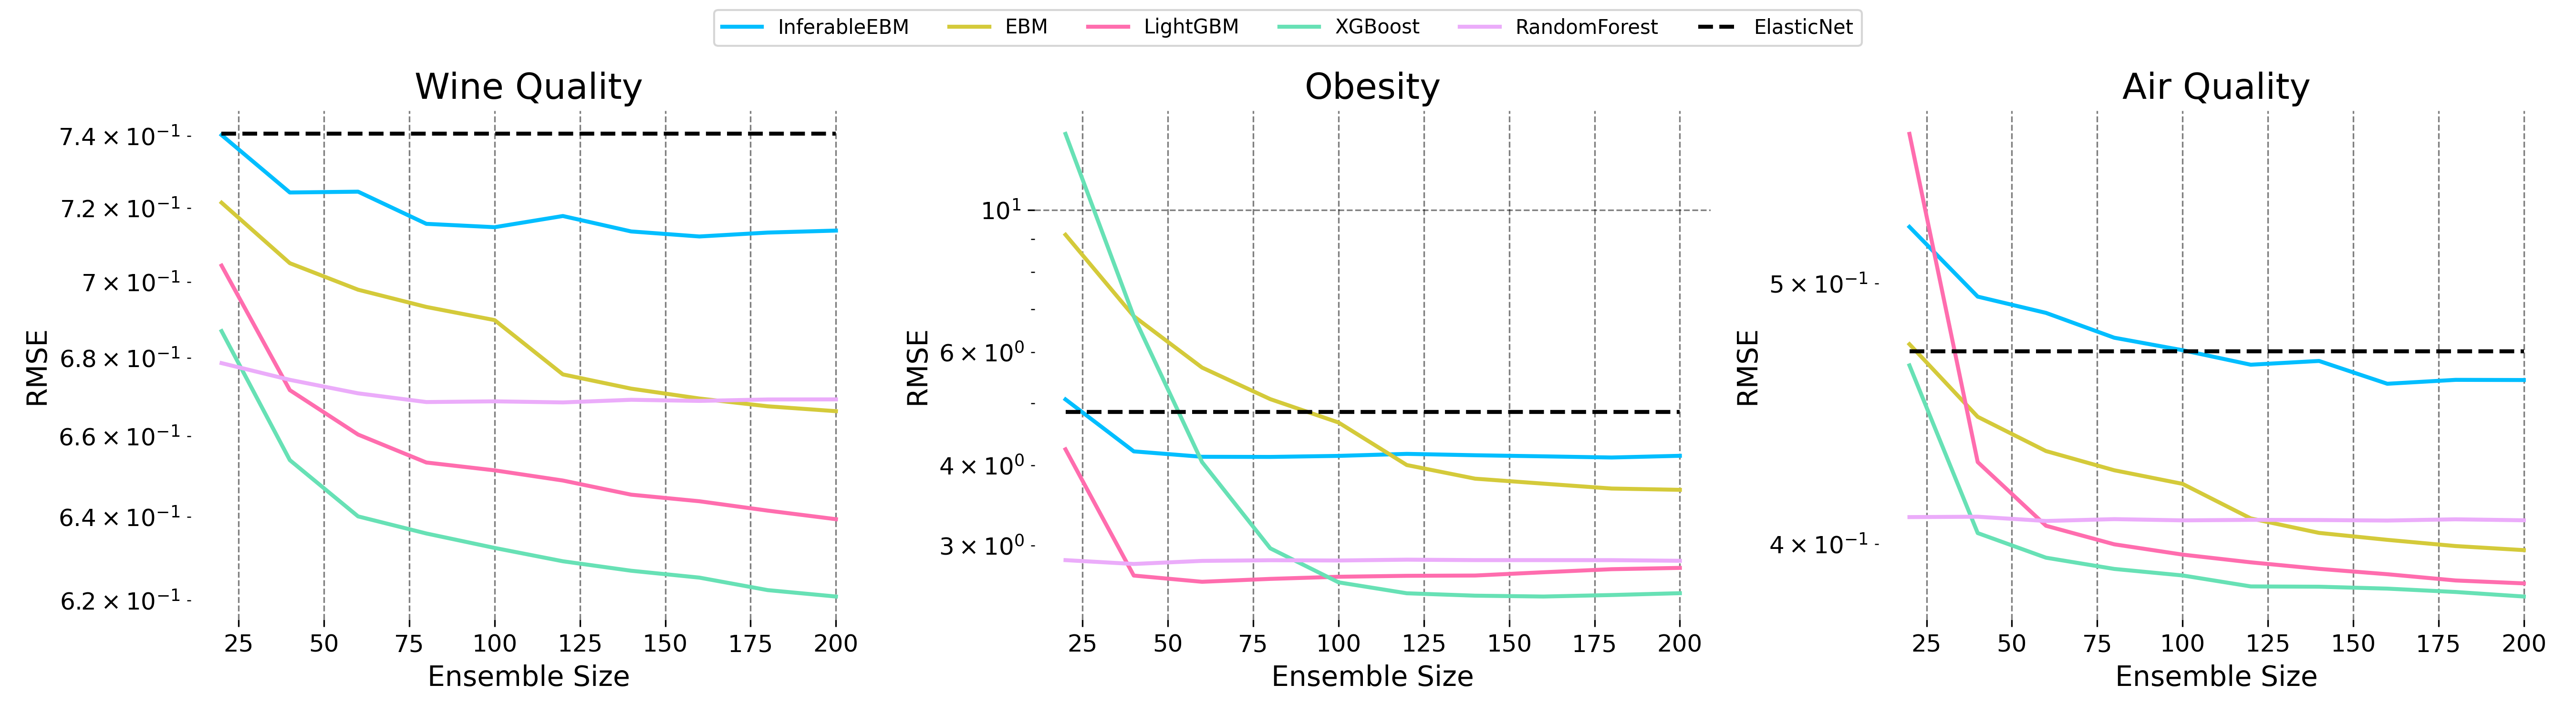
\includegraphics[width=0.85\linewidth]{figures/ch06/plots_ebm/optuna_mse.png}\vspace{-2ex}
        \caption{MSE horse races on UCI machine learning repository datasets. All hyperparameters tuned by Optuna.}
        \label{fig:mse-horse-races}
    \end{figure*}
    \addtocounter{figure}{-1}
    
	\subsection{Numerical Experiments}
    \label{ch06b:sec:experiments}
    \paragraph{Predictive Accuracy} We compare Algorithm \ref{alg:brebm_ident} to other benchmark models on real world data from the UCI Machine Learning Repository in Figure \ref{fig:mse-horse-races}. Algorithm \ref{alg:brebm_ident} is competitive with EBMs across the Wine Quality, Obesity and Air Quality datasets, while converging much faster with parallelization. However, these datasets exhibit higher order interactions. Algorithm \ref{alg:brebm_ident} and EBMs ultimately underperform random forests and gradient boosting, though their added flexibility allows them to outperform a linear model. 
    
    However, the above setup had hyperparameters extensively tuned by Optuna over 100 trials. When this is not feasible, gradient boosting can be susceptible to overfitting. Figure \ref{fig:overfit_mse} depicts two examples where this is the case, on $f(x) = \sin(4\pi x)$ and the diabetes dataset from \cite{Efron_2004}. Here, the performances are flipped. Algorithm \ref{alg:brebm_ident} and EBMs perform the best with no need for early stopping, while the gradient boosting methods quickly overfit. EBMs achieve this via a tiny learning rate during cyclic boosting, while our implementation parallelizes over features for faster runtime.
    
    \paragraph{Interval Coverage Rates} To validate the proposed central limit theorems, we first construct feature-wise confidence intervals via binning and compute their coverage rates. Figure \ref{fig:feature-coverage} shows good coverage and width. In combination with Figure \ref{fig:coverage-1d}, we can qualitatively argue that their performance appears desirable.

    Figure \ref{fig:ebm-effects-wide} and Figure \ref{fig:obesity-feature-effects} yield an example on real-world data from the obesity dataset of \cite{estimation_of_obesity_levels_based_on_eating_habits_and_physical_condition__544}, regressing weight on other covariates. Our intervals offer much-needed uncertainty estimates for each effect.
    
    Figure \ref{fig:coverage-rates} compares the coverage and width of the CIs and PIs for the overall response, and RIs for another realization. We use the same conformal correction that \cite{fang2025gradient} use for the PIs only. Coverage is close to nominal for the CIs and PIs, while the RIs exhibit some overcoverage. 

    We further evaluate scalability in higher-dimensional, correlated synthetic additive models for Algorithm~\ref{alg:ebm_bratp} under the realistic Assumption~\ref{aspt:kernel-spec}. In Figure~\ref{tab:vanilla_vs_inferable_gam}, bootstrap EBMs achieve low RMSE but severely under-cover and are slow due to repeated refits, while Algorithm~\ref{alg:ebm_bratp} (and BRATD) attain near-nominal coverage; moreover, Algorithm~\ref{alg:ebm_bratp} yields better RMSE and tighter intervals than BRATD at comparable or lower runtime. Compared with \cite{fang2025gradient}, our intervals are also faster and better-behaved, since we avoid the curse of dimensionality and our runtime is independent of $n$.

    
    
    Figure \ref{fig:highdim-real-table} shows that on real datasets with $p\approx 110$--$130$, Algorithm~\ref{alg:ebm_bratp} maintains near-nominal $95\%$ coverage ($0.948$--$0.956$), achieves RMSE comparable to the baselines, and is substantially faster than vanilla EBM. Relative to BRATD, it attains similar RMSE with lower training time on three of the four datasets, especially on the largest example.

    \addtocounter{figure}{-1}
	\begin{figure}[H]
		\hspace{-3ex}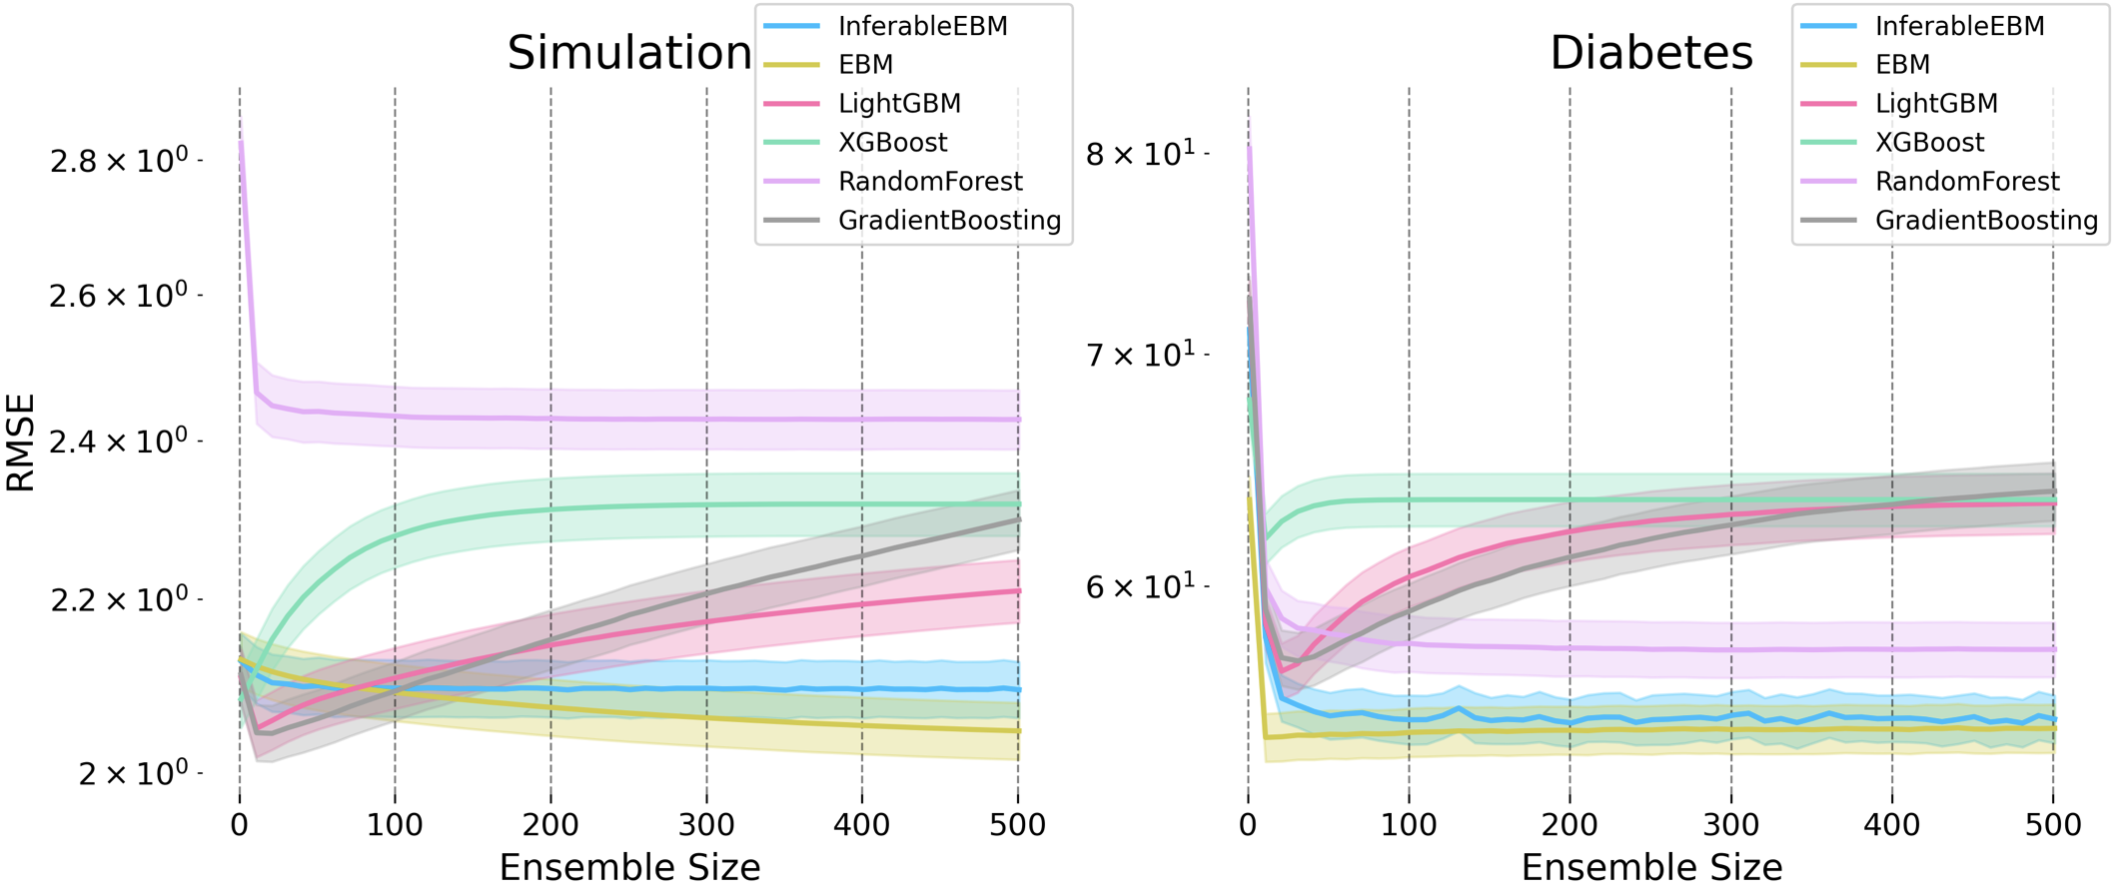
\includegraphics[width=1.1\linewidth]{figures/ch06/plots_ebm/overfit_combined.png}
		\caption{RMSE for Algorithm \ref{alg:brebm_ident} and benchmarks with 2 s.e. bands over 50 trials, on $f(x) = \sin(4\pi x)$ and the diabetes dataset from \cite{Efron_2004}. Both EBM and Algorithm \ref{alg:brebm_ident} are highly resistant to overfitting.}
		\label{fig:overfit_mse}
	\end{figure}
    \addtocounter{figure}{1}

    \subsection{Conclusion}
	Explainable boosting machines have been an important tool for producing glass-box models, used both to establish insight into the underlying patterns that generate data, and to diagnose potential non-causal behavior prior to deployment. The understanding presented by such methods must be qualified by appropriate uncertainty quantification. Current UQ for EBMs relies on bootstrapping which is both computationally intensive and lacks theoretical backing.
    
    \begin{figure}[H]
        \hspace{-3ex}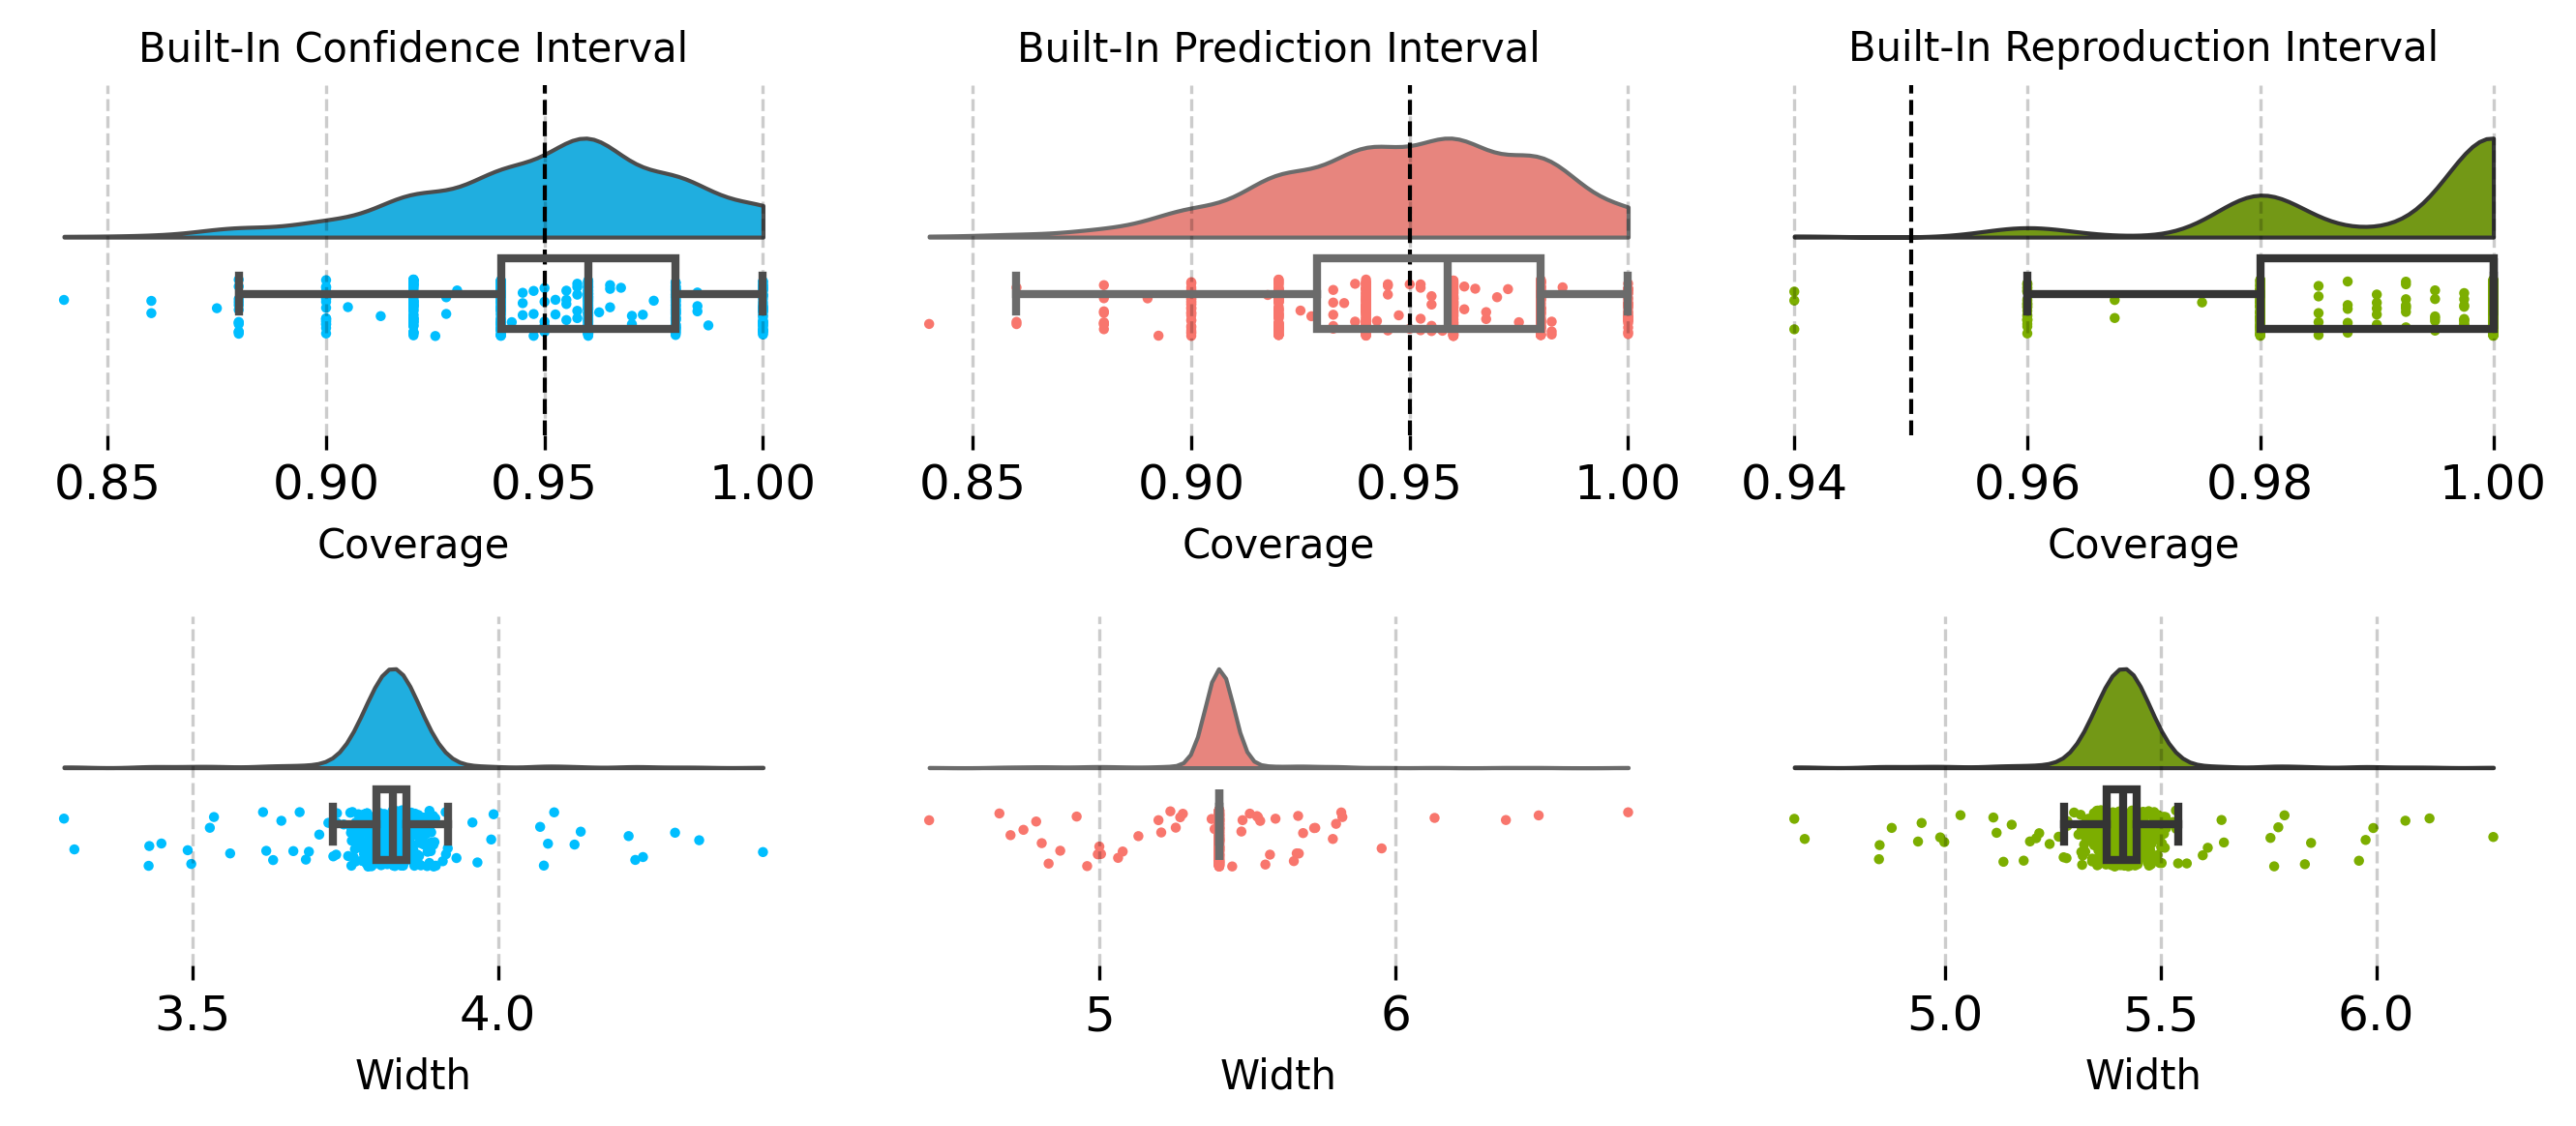
\includegraphics[width=1.0\linewidth]{figures/ch06/plots_ebm/coverage_rates.png}
        \caption{Coverage and width of our intervals over $50$ trials, $n=2000$, on the same function as Figure \ref{fig:feature-coverage}.}
        \label{fig:coverage-rates}
    \end{figure}

    The Boulevard regularization method that we adopt to EBM here both removes the need to choose stopping times (see Figure \ref{fig:overfit_mse}), and generates a limit that can be characterized as a kernel ridge regression. This enables us to directly derive a central limit theorem for predictions of the resulting model and their additive components, and to thereby both derive consistent estimates of their asymptotic variance and provide confidence intervals and tests. 

    This work opens several extensions.  We can readily extend the function class to more complex additive structure; including isolated interaction terms is straightforward, although additive components with shared features require new identifiability conditions \cite[e.g.][]{lengerich2020purifying}. More generally, these methods are extensible to mixtures of learners, such as the class of varying coefficient models discussed in \citet{zhou2022decision}. We can an also broaden the class of models to discrete outcomes and models with non-constant variance. Finally, the kernel form of the limit also admits combinations and comparisons across models as described in \cite{ghosal2022infinitesimal}.
    
    \begin{table}[H]
    \centering
    \scriptsize
    \setlength{\tabcolsep}{3.2pt} % tighten columns to fit one column
    \renewcommand{\arraystretch}{1.15} % add vertical breathing room
    
    \begin{tabular}{c l c c c c}
        \toprule
        $p$ & Method & RMSE & Coverage & Width & Time (s) \\
        \specialrule{0.6pt}{0.35em}{0.35em}
        
        \multirow{3}{*}{5}
        & Bootstrap EBM                    & 0.514 & 0.290 & 0.386 & 26.42 \\
        & Algorithm~\ref{alg:ebm_bratp}     & 0.661 & 0.951 & 2.609 &  3.00 \\
        & BRATD                            & 0.611 & 0.956 & 2.899 & 10.41 \\
        \specialrule{0.6pt}{0.35em}{0.35em}
        
        \multirow{3}{*}{10}
        & Bootstrap EBM                    & 0.537 & 0.373 & 0.545 & 21.24 \\
        & Algorithm~\ref{alg:ebm_bratp}     & 0.788 & 0.951 & 3.069 &  5.90 \\
        & BRATD                            & 0.866 & 0.935 & 3.531 & 13.58 \\
        \specialrule{0.6pt}{0.35em}{0.35em}
        
        \multirow{3}{*}{15}
        & Bootstrap EBM                    & 0.563 & 0.453 & 0.675 & 31.51 \\
        & Algorithm~\ref{alg:ebm_bratp}     & 0.900 & 0.945 & 3.520 &  8.77 \\
        & BRATD                            & 1.112 & 0.946 & 4.398 & 10.29 \\
        \specialrule{0.6pt}{0.35em}{0.35em}
        
        \multirow{3}{*}{20}
        & Bootstrap EBM                    & 0.583 & 0.511 & 0.801 & 43.14 \\
        & Algorithm~\ref{alg:ebm_bratp}     & 1.004 & 0.948 & 3.901 & 11.56 \\
        & BRATD                            & 1.332 & 0.948 & 5.121 & 10.70 \\
        \bottomrule
    \end{tabular}
    
    \vspace{0.25em}
    \caption{Synthetic Lipschitz GAMs (bootstrap EBM vs.\ Algorithm~\ref{alg:ebm_bratp} vs.\ BRATD).
    Synthetic additive model with $n=1000$ and $p\in\{5,10,15,20\}$ (all $p$ features are structural; five base univariate functions are cycled across coordinates):
    $f_1(x)=2\sin(\pi x)$, $f_2(x)=(x-0.5)^2$, $f_3(x)=0.5\times\mathbf{1}\{x>0.3\}$, $f_4(x)=\sqrt{x}$, $f_5(x)=-1.5x$.
    We report mean RMSE, model-level empirical coverage at nominal $95\%$, average interval width, and runtime (seconds) over 10 repetitions ($\alpha=0.05$; 250 bootstrap resamples for EBM).}
    
    \label{tab:vanilla_vs_inferable_gam}
    \end{table}

    \begin{table}[H]
    \centering
    \scriptsize
    \setlength{\tabcolsep}{3.5pt}

    % ---- Table A: Algorithm 2 (inference + training) ----
    \begin{tabular}{@{}l r r c c c@{}}
        \toprule
        Dataset & $n$ & $p$ &
        \begin{tabular}[c]{@{}c@{}}RMSE\\(Alg.~\ref{alg:ebm_bratp})\end{tabular} &
        \begin{tabular}[c]{@{}c@{}}Cov.\\(Alg.~\ref{alg:ebm_bratp})\end{tabular} &
        \begin{tabular}[c]{@{}c@{}}Time (s)\\(Alg.~\ref{alg:ebm_bratp})\end{tabular} \\
        \midrule
        taiwanese\_bankruptcy   &  6819 &  95  & 0.151 & 0.948 & 18.01 \\
        myocardial\_infarction  &  1700 & 111  & 0.309 & 0.943 &  3.53 \\
        communities\_and\_crime &  1994 & 127  & 0.140 & 0.953 &  5.68 \\
        dota2\_results          & 50000 & 116  & 0.142 & 0.956 & 28.78 \\
        \bottomrule
    \end{tabular}

    \vspace{0.35em}

    % ---- Table B: Baseline accuracy/runtime (training) ----
    \begin{tabular}{@{}l c c c c@{}}
        \toprule
        Dataset &
        \begin{tabular}[c]{@{}c@{}}RMSE\\(EBM)\end{tabular} &
        \begin{tabular}[c]{@{}c@{}}Time (s)\\(EBM)\end{tabular} &
        \begin{tabular}[c]{@{}c@{}}RMSE\\(BRATD)\end{tabular} &
        \begin{tabular}[c]{@{}c@{}}Time (s)\\(BRATD)\end{tabular} \\
        \midrule
        taiwanese\_bankruptcy   & 0.153 &  197.31 & 0.154 & 24.58 \\
        myocardial\_infarction  & 0.309 &   52.62 & 0.311 &  3.78 \\
        communities\_and\_crime & 0.135 &  178.41 & 0.144 &  7.80 \\
        dota2\_results          & 0.013 & 3736.10 & 0.147 & 82.62 \\
        \bottomrule
    \end{tabular}

    \caption{We report RMSE, $95\%$ empirical coverage, and training time for Algorithm~\ref{alg:ebm_bratp} (top), and baseline RMSE and training time for vanilla EBM and BRATD (bottom). Baseline coverage is omitted because large-scale uncertainty estimation is not computationally scalable.}
    \label{fig:highdim-real-table}
    \end{table}
	
	
	